Using the reconstructed objects discussed in the previous chapter, 
we can select the Higgs events by selecting events with two leptons 
and \met. But, the selected events contain not only signal, 
but also backgrounds. A challege is that the production rate 
of the backgrounds is much larger than that of signal. 
\begin{figure}[htp] 
\centering 
\begin{tabular}{c} 
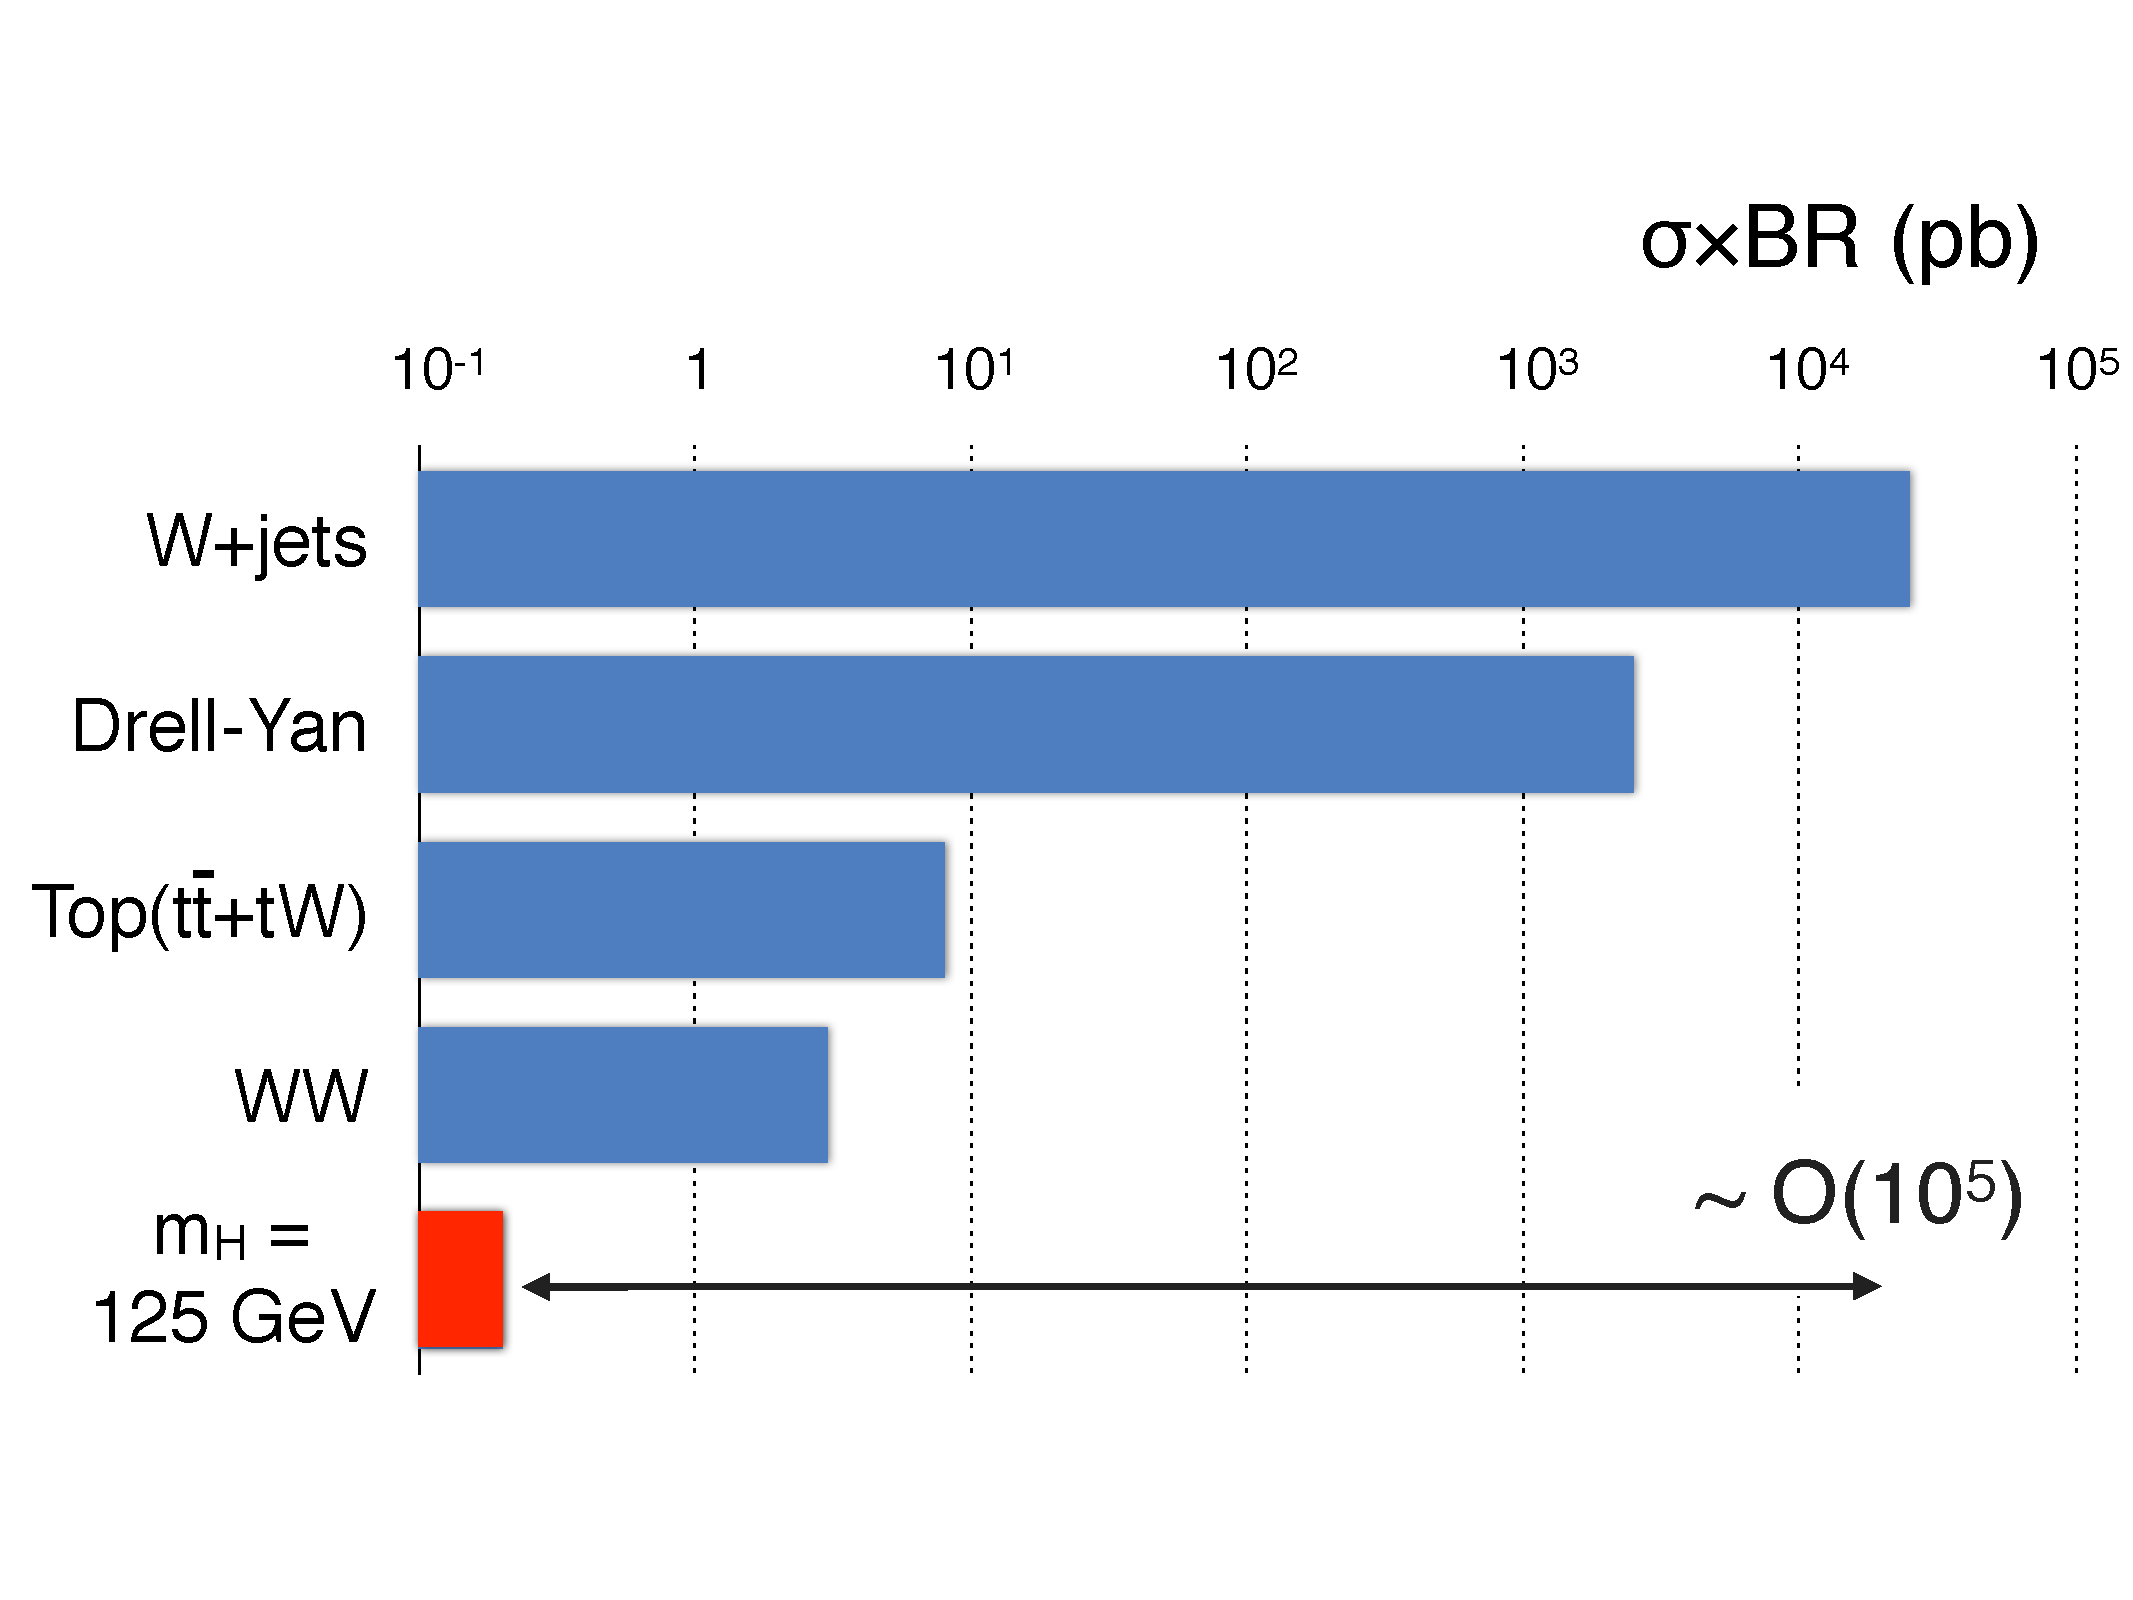
\includegraphics[width=0.95\textwidth]{figures/BkgProdRate.pdf} 
\end{tabular} 
\caption{The cross section $\times$
branching ratio($\sigma \times BR$) for the major background
processes and the SM \mHi=125~\GeV\ hypothesis. The branching ratio
is for the leptonic decay(electron/muon + neutrino) of W or Z.} 
\label{fig:bkgprodrate} 
\end{figure} 
Fig.~\ref{fig:bkgprodrate} shows the cross section $\times$ 
branching ratio($\sigma \times BR$) for the major background 
processes and the SM \mHi=125~\GeV\ hypothesis. 
The production rate of backgrounds is much larger than the signal. 
For example, the $\sigma \times BR$ of the \Wjets\ is a factor of 
$\mathcal{O}(10^5)$ larger than that of signal.  
Therefore, we need to apply stringent requirements which 
select the signal events with high efficiency, and suppress 
background events with a high rejection rate.  

The backgrounds can be divided into two categories depending on 
the way they can be suppressed. The first kind is reducible 
backgrounds which can be suppressed by tighting the requirements 
on the object selection. The reducible backgrounds are 
\dyll, \topbkg, \Wjets, \wgamma, \wgammastar, \vv\ and \ztt\
where for \vv\ there are more than 2 leptons in the final state.  
The other kind is irreducible backgrounds 
which have the exactly same final states as signal, 
therefore they can not be suppressed by tightening object selections,  
but by using event kinematics. The irreducible backgrounds 
are \ww\ and \vv\ where for \vv\ there are only 2 leptons 
in the final state, \textit{e.g.}, missing leptons. 

This chapter describes the selection criteria to suppress the
reducible backgrounds. The requirements are imposed to 
trigger, vertex, electron, muon, jets, and top-tagging selections. 
In addition, there are requirements to suppress 
particular backgrounds. All these requirements are designed 
to select events containing a pair of Ws to make a subset of 
sample with a reasonable signal-to-background ratio for 
signal extraction. The next chapter describes the selection 
to suppress irreducible backgrounds to extract the signal events. 


%%%%%%%%%%%%%%%%%%%%%%%%%%%%%%%%%%%%%%%%%%%%%%%%%%%%%%%%%%%%%%%%%%
\section{Trigger}
\label{sec:trigger}

As discussed in section~\ref{subsec:kinimetic_variables}, 
\hww\ events have trailing lepton 
whose transverse momentum goes down very low for low \mHi\ hypotheses. 
But, triggering low 
\pt\ leptons is very challenging because of large background events. 
Therefore, in order to record signal events with high efficiency, 
we need to trigger on the leading lepton, 
or on both leptons. The option to trigger on the leading lepton 
is not possible because the requirements should be very tight 
to maintain a sustainable bandwidth. Thus, we trigger on both leptons. 
The double-lepton triggers we designed for this analysis have high efficiency for  
signal events, but are loose enough to collect events in the several control regions 
we use for various studies. We also use control region triggers that allow 
fake rate and lepton selection efficiency measurements which are described 
in section~\ref{sec:wjets} and~\ref{sec:lepeff}, respectively,
with a precision good enough for this analysis. 

%\textcolor{red}{Where can I check the bandwidth of triggers? want to know 
%the total bandwidth of~\cmS and the bandwidth of triggers we use}

\subsection{Analysis Triggers}

The analysis triggers, the triggers used to select signal and control region events, 
impose tight cuts to maintain the rate. 
For the electron HLT objects there are requirements on
the kinematics(\pt\ and \Eta), 
the shower shapes, %(H/E, $\sigma_{\eta\eta}$), 
the track-to-cluster matching and 
%($|\Delta\eta|$, $|\Delta\phi|$, $|\frac{1}{E}-\frac{1}{p}|$),
the track/calorimeter isolation. %(ECalIso, HCalIso, TrkIso). 
For the muon HLT objects there are requirements on 
the kinematics(\pt\ and \Eta). 
The naming convention and the corresponding 
cut variables with their cut values are listed in Table~\ref{tab:trg_requirement_def}.
%
\begin{table}[!ht]
 \centering
 \begin{tabular}{l|c}
   \hline
   name                       &  criterion \\
   \hline \hline
   \multirow{2}{*}{CaloId\_T} & $\mathrm{H/E < 0.15 (0.10) }$ \\
                               & $\sigma_{\eta\eta}\mathrm{< 0.011\;(0.031)}$ \\
    \hline
   \multirow{2}{*}{CaloId\_VT} & $\mathrm{H/E < 0.05 (0.05) }$ \\
                               & $\sigma_{\eta\eta}\mathrm{< 0.011\;(0.031)}$  \\
    \hline \hline
    \multirow{2}{*}{TrkId\_VL} & $|\Delta\eta|\mathrm{< 0.01\; (0.01)}$ \\
                               & $|\Delta\phi|\mathrm{< 0.15\;(0.10)}$  \\
    \hline
    \multirow{2}{*}{TrkId\_T} & $|\Delta\eta|\mathrm{< 0.008\; (0.008)}$ \\
                              & $|\Delta\phi|\mathrm{< 0.07\;(0.05)}$ \\
    \hline \hline
    \multirow{2}{*}{CaloIso\_VL} & $\mathrm{ECalIso/E_T <0.2\;(0.2)}$ \\
                                 & $\mathrm{HCalIso/E_T <0.2\;(0.2)}$ \\
    \hline
    \multirow{2}{*}{CaloIso\_T} & $\mathrm{ECalIso/E_T <0.15\;(0.075)}$ \\
                                 & $\mathrm{HCalIso/E_T <0.15\;(0.075)}$ \\
    \hline
    \multirow{2}{*}{CaloIso\_VT} & $\mathrm{ECalIso/E_T <0.05\;(0.05)}$ \\
                                 & $\mathrm{HCalIso/E_T <0.05\;(0.05)}$ \\
    \hline \hline
    TrkIso\_VL                   & $\mathrm{TrkIso/E_T <0.2\;(0.2)}$ \\
    \hline
    TrkIso\_T                   & $\mathrm{TrkIso/E_T <0.15\;(0.075)}$ \\
    \hline
    TrkIso\_VT                   & $\mathrm{TrkIso/E_T <0.05\;(0.05)}$ \\
    \hline \hline
    \multirow{8}{*}{WP80} 		& $\mathrm{H/E < 0.10 (0.05) }$ \\
                               	& $\sigma_{\eta\eta}\mathrm{< 0.01\;(0.03)}$ \\
    							& $|\Delta\eta|\mathrm{< 0.007\; (0.007)}$ \\
                               	& $|\Delta\phi|\mathrm{< 0.06\;(0.03)}$  \\
                               	& $|\frac{1}{E}-\frac{1}{p}|\mathrm{< 0.05\;(0.05)}$  \\
    							& $\mathrm{ECalIso/E_T <0.15\;(0.10)}$ \\
                                & $\mathrm{HCalIso/E_T <0.10\;(0.10)}$ \\
                       			& $\mathrm{TrkIso/E_T <0.05\;(0.05)}$\\
    \hline
 \end{tabular}
 \caption{Summary of requirements applied to electrons in the analysis triggers.
The selection requirements are shown for electrons in the barrel (endcap).
The abbreviation in the names means L=Loose, VL=Very Loose, T=Tight, and VT=Very Tight.}
 \label{tab:trg_requirement_def}
\end{table}
The H/E is the ratio of energy deposit in HCAL to that of ECAL. 
The $\sigma_{\eta\eta}$ is the weighted sum of \Eta\ difference between the 
seed crystal and the 5x5 crystals surrounding it.   
The $|\Delta\eta|(|\Delta\phi|)$ is the difference in absolute value between 
the center of the supercluster and the direction of the track trajectory 
in \Eta($\phi$) direction.   
The $|\frac{1}{E}-\frac{1}{p}|$ is the difference between 
the reciprocal of supercluster energy 
and the reciprocal of the track momentum.  
The $\mathrm{ECalIso/E_T}$, $\mathrm{HCalIso/E_T}$ and $\mathrm{TrkIso/E_T}$ 
are the sum of the transverse energy within $dR<0.3$ % \textcolor{red}{(checked)} 
around the center of the energy deposit or the track trajectory
divided by the transverse energy, $\mathrm{E_T}$.
The details of these variables are discussed in section~\ref{sec:electron}.
% E_T(SC) for Ecal, and elecand.pt() for Hcal and Tk (guess this is track momentum)  

In this analysis we use double-lepton triggers as shown in Table~\ref{tab:trg_doublelepton} 
and single-lepton triggers as shown in Table~\ref{tab:trg_singlelepton}.
\begin{table}[!ht]
  \centering 
  \begin{tabular} {l|l}
  \hline
  Double-lepton trigger name & L1 seed \\
  \hline \hline
  HLT\_Ele17\_CaloIdT\_CaloIsoVL\_TrkIdVL\_TrkIsoVL\_ 	    &  L1\_DoubleEG\_13\_7  \\
  Ele8\_CaloIdT\_CaloIsoVL\_TrkIdVL\_TrkIsoVL\_v[15-19] 	&                       \\ 
  %190456-190738 %190762-191419 %191512-194533
  \hline
  HLT\_Mu17\_Mu8\_v[16-22] 	    & L1\_DoubleMu\_10\_Open    \\ %190456-193686 %193806-194533
  HLT\_Mu17\_TkMu8\_v[9-14] 	& OR L1\_DoubleMu\_10\_3p5  \\ %190456-193686 %193806-194533
  \hline
  HLT\_Mu17\_Ele8\_CaloIdT\_CaloIsoVL\_ 	& L1\_Mu12\_EG7     \\
  TrkIdVL\_TrkIsoVL\_v[4-9] 	            &     \\
  %190456-190738 %190762-191419 %191512-193686 %193806-194533
  HLT\_Mu8\_Ele17\_CaloIdT\_CaloIsoVL\_	    & L1\_MuOpen\_EG12       \\ 
  TrkIdVL\_TrkIsoVL\_v[4-9] 	            & OR L1\_Mu3p5\_EG12     \\ 
  %190456-190738 %190762-191419 %191512-193686 %193806-194533
  \hline
  \end{tabular} 
  \caption{Double-lepton triggers used to collect signal events. 
           The naming convention is shown in Table~\ref{tab:trg_requirement_def}.} 
  \label{tab:trg_doublelepton}
\end{table}
%
\begin{table}[!ht]
  \centering 
  \begin{tabular} {l|l}
  \hline
  Single-lepton trigger name & L1 seed \\
  \hline \hline
  HLT\_Ele27\_WP80\_v[8-11] & L1\_SingleEG20 OR L1\_SingleEG22  \\ 
  %190456-190738 %190762-191419 %191512-194533
  \hline 
  HLT\_IsoMu24\_eta2p1\_v[11-15]   & L1\_SingleMu16er  \\  
  %190456-190738 %190762-193686 %193806-194533
  \hline \hline
  \end{tabular}
  \caption{Single-lepton triggers used to collect signal events. 
           The naming convention is shown in Table~\ref{tab:trg_requirement_def}.} 
  \label{tab:trg_singlelepton}
\end{table}
The double-lepton triggers require two HLT objects to be present, 
and each of them is required to match an L1 seed. The offline lepton \pt\ 
requirement is 20/10~\GeV, so the online lepton \pt\ requirement is a bit looser, 17/8~\GeV, 
in order to be avoid loosing events by online selection. In addition,
the longitudinal distance between the two vertices of the leptons is required 
to be less than 0.2~\cm\ in order to ensure that the two leptons are 
coming from the same interaction point. The requirement of the single lepton triggers 
is tighter than that of double-lepton triggers to maintain the bandwidth. 
Single-lepton triggers help enhance the overall trigger efficiency 
by selecting events that the double-lepton triggers missed. 

Because online variables are constructed using more simplified algorithms 
than the offline variables, they do not exactly correspond to the offline ones. 
To account for this, we measure the trigger efficiency with respect to the 
offline selection, and apply corrections accordingly. 
The details on this can be found in~\ref{subsec:trg_eff} where the 
measurement on the trigger efficiency is discussed.
%\textcolor{red}{what is TkMu8? what is the iso requirement on single muon triggers?} 


\subsection{Utility Triggers}

The efficiency measurements of the lepton selection  
are performed by \tnp\ method~\cite{Abulencia:2005ix} using \dyll\ events. 
In order to use this method, we select a pure sample 
of \dyll\ events to reduce bias due to selecting non-prompt leptons from 
other background processes or pileup. Apart from the analysis triggers, for this 
measurement we do not have to select all available events, but a pure sample with 
an adequate statistics. The single lepton triggers used to collect signal events, 
listed in Table~\ref{tab:trg_singlelepton}, also can be used to select 
\dyll\ events. The leading lepton is likely to be triggered, making the 
trailing lepton unbiased sample that covers a wide range of 
kinematic region that stretches to low lepton \pt.   

In order to estimate jet-induced backgrounds such as \Wjets\ that have a non-prompt 
lepton that passes the full lepton selection, we use ``fake rate" method.  
The details of this method are discussed in~\ref{sec:wjets}. 
In this method we define a loose lepton selection, and calculate the ratio, 
``fake rate", for a lepton that pass a loose selection to pass the full selection, 
using a data sample of single-lepton events dominated by QCD processes. 
The assumption of this method is that the jets in \Wjets\ events 
and QCD events are not different, and the fake rate measured using the two samples is same. 
This is possible only if the kinematics, particularly \pt, of the progenitor 
of the jets are same~\footnote{Consider a fake lepton of \pt=20~\GeV. 
The fake rate in case that the progenitor \pt=25~\GeV(a) is 
different from the case that the progenitor \pt=100~\GeV(b). 
(b) has more extra energy (100 - 20 = 80~\GeV) than (a), 
so it has larger probability to be un-isolated giving lower fake rate.
Other issue is the composition of the progenitor in the two samples,
\textit{e.g.} gluon-quark ratio and quark flavor, 
but this is a second-order effect.}.
In data, we do not have a handle to control the \pt\ of the progenitor,
so we use the \pt\ of the jet that is on the other side of the lepton(away jet).  
This is justified by the fact that QCD events are dominated by 
di-jet events where the two jets are likely to be back-to-back. 
By choosing an appropriate \pt\ cut of the away jet, 
we can select relevant event samples to measure fake rate
and the systematic uncertainty due to limitation of controlling 
the progenitor \pt\ is covered by varying the away jet \pt\ threshold.


Because the leptons in the data sample collected by the analysis triggers 
are also trigger objects, the loosest possible 
``loose" definition is the trigger requirement of the analysis triggers.
We devised a set of single-lepton triggers that have a loose or the same requirements 
on leptons as the double-lepton triggers. 
%Note that the single lepton triggers have tighter requirements on leptons. 
In order to cover large range of lepton \pt, 
we use several triggers with different lepton \pt\ thresholds.
In addition, as fake rate is measured with a \pt\ cut on the away jet 
we can obtain more events in the relevant phase space
by applying \pt\ cut on the away jet. 
The single lepton triggers used for fake rate measurement are listed in 
Table~\ref{tab:triggers_fr}. These triggers provide sufficient statistics 
for measurement of fake rate and estimation of its systematic uncertainty.     

%For the data-driven estimation for \dyll\ backgrounds we have alternate method 
%that uses photon + jets events. These events are triggered by photon triggers 
%and the photon triggers used for this analysis are listed in the Table~\ref{tab:}.


\begin{table}[!ht]
  \begin{center}
 {\small
  \begin{tabular} {l|l}
\hline
 Trigger name & L1 seed \\
\hline\hline
 HLT\_Ele8\_CaloIdT\_TrkIdVL\_v[2-5]	& L1\_SingleEG5 		\\ %190456-190738 %190762-191419 %191512-194533
 HLT\_Ele8\_CaloIdT\_CaloIsoVL\_		& L1\_SingleEG7 		\\ 
 TrkIdVL\_TrkIsoVL\_v[12-15]			&  						\\ %190456-190738 %190762-191419 %191512-194533
 HLT\_Ele17\_CaloIdT\_CaloIsoVL\_  		& L1\_SingleEG12		\\ 
 TrkIdVL\_TrkIsoVL\_v[3-6]  			& 						\\ %190456-190738 %190762-191419 %191512-194533
 HLT\_Ele8\_CaloIdT\_CaloIsoVL\_      	& L1\_SingleEG7         \\
 TrkIdVL\_TrkIsoVL\_Jet30\_v[3-7]      	& 						\\ %190456-190738 %190762-191419 %191512-194533
 HLT\_Ele17\_CaloIdT\_CaloIsoVL\_		& L1\_SingleEG12		\\ 
 TrkIdVL\_TrkIsoVL\_Jet30\_v[3-7]		& 						\\ %190456-190738 %190762-191419 %191512-194533
	\hline \hline
 HLT\_Mu8\_v[16-18] 	&  L1\_SingleMu3  		\\ %190456 - 194533
 HLT\_Mu17\_v[3-5]      &  L1\_SingleMu12   	\\ %190456 - 194533   
%	\hline \hline
% HLT\_Photon22\_R9Id90\_HE10\_Iso40\_EBOnly\_v[2-4]					& L1\_SingleEG22		\\ %190456-190738 190762-191419 %191512-194731
% HLT\_Photon36\_R9Id90\_HE10\_Iso40\_EBOnly\_v[2-4]					& L1\_SingleEG22		\\ %190456-190738 190762-191419 %191512-194731
% HLT\_Photon50\_R9Id90\_HE10\_Iso40\_EBOnly\_v[2-4]					& L1\_SingleEG22		\\ %190456-190738 190762-191419 %191512-194731
% HLT\_Photon75\_R9Id90\_HE10\_Iso40\_EBOnly\_v[2-4]					& L1\_SingleEG22		\\ %190456-190738 190762-191419 %191512-194731
% HLT\_Photon90\_R9Id90\_HE10\_Iso40\_EBOnly\_v[2-4]					& L1\_SingleEG22		\\ %190456-190738 190762-191419 %191512-194731
    \hline 
  \end{tabular}
}
  \caption{Utility triggers for fake rate method. %and zeta method. 
  The identification and isolation requirements for electrons are described in Table~\ref{tab:trg_requirement_def}. 
  Jet30 in the electron triggers means that there should be at least one jet of $\pt>30~\GeV$.
%The identification and isolation requirements for photons are described in Table~\ref{tab:PhotonPlusLeptonTriggerCuts}.
}
%and ``$\zeta$ method " are used for Drell-Yan background estimation.}
   \label{tab:triggers_fr}
  \end{center}
\end{table}

%
%\begin{table}[htb]
%  \centering
%  \begin{tabular}{l|c}
%    \hline
%    name                        &  criterion \\
%    \hline \hline 
%    \multirow{1}{*}{R9Id90} 	& $\mathrm{R9 > 0.9 }$ \\
%    \hline 
%    \multirow{1}{*}{HE10} 		& $\mathrm{H/E < 0.1 }$ \\
%    \hline 
%    \multirow{3}{*}{Iso40}     	& $\mathrm{ECalIso} < 4.0 $ \\
%                                & $\mathrm{HCalIso} < 4.0 $ \\
%                                & $\mathrm{TrkIso}  < 4.0 $ \\
%    \hline 
%  \end{tabular}
%   \caption{Summary of requirements applied in the photon triggers used for this analysis.}
%   \label{tab:trg_requirement_def_photon}
%\end{table}

%%%%%%%%%%%%%%%%%%%%%%%%%%%%%%%%%%%%%%%%%%%%%%%%%%%%%%%%%%%%%%%%%%
\section{ Event Primary Vertex }
%\begin{itemize}
%\item \textcolor{red}{Track reconstruction : Kalman Filter, ...}
%\item \textcolor{red}{Vertex reconstruction : vertex finding, vertex fitting, ...}
%\item \textcolor{red}{Primary Vertex selection}
%\end{itemize}

The offline primary vertices are required to be within 24~\cm\ from the center of the 
detector 
%\textcolor{red}{(or beamspot?)} 
in z direction. 
It should be within 2~\cm\ from the beam spot in the radial direction. 
The degrees of freedom of the vertex fit should be 4 or larger. 
%\textcolor{red}{what does this mean exactly?} 

At high luminosity collisions, there are multiple proton-proton interactions 
in the same bunch crossing. In those interactions there is usually 
only one interaction that is of interest for our analysis, which triggered that event. 
These interactions tend to be associated with energetic objects, 
while the other interactions are mostly inelastic scatterings that produce soft objects.
Therefore, we choose the event primary vertex by selecting the primary vertex 
with the largest scalar sum of $\pt^2$ of tracks associated with the vertex. 
%The vertices of leptons are required to be very close to the event primary vertex.  



%%%%%%%%%%%%%%%%%%%%%%%%%%%%%%%%%%%%%%%%%%%%%%%%%%%%%%%%%%%%%%%%%%
\section{ Electron }
\label{sec:electron}

An electron candidate is reconstructed if there is a track and a supercluster energy 
deposit compatible with the track momentum. There are multiple sources of 
electrons which do not originate from hard interactions. These electrons 
are called ``non-prompt electrons" as opposed to the 
``prompt electrons" originated from hard interactions. 
Of the non-prompt electrons, those that originate from jets is called ``fake electrons or fakes".
We can get fake electrons if  
\begin{itemize}
\item Early conversion : $\pi^0$ decays to two photons, and one of the two photons
      undergoes an asymmetric conversion to an electron-positron pair, \textit{i.e.}, 
      one of the them carries most of the photon momentum,
\item Charge exchange : $\pi^\pm$ is converted to $\pi^0$ in the ECAL, 
      and the $\pi^0$ decays to a pair of photons,
\item Random combination : $\pi^\pm$ overlaps $\pi^0$(a track of $\pi^\pm$ 
      randomly matches a supercluster energy deposit by $\pi^0$), and 
\item Heavy flavor decay : B or D hadron decays semi-leptonically.  
\end{itemize}
In order to suppress fake electrons, we apply selections composed of 
requirements on the identification,
%(track-to-supercluster matching, 
%track fit quality, shower shape, energy loss due to \brem\, ratio of hadronic energy
%to electromagnetic energy), 
isolation and impact parameter.  
Other source of non-prompt electrons is a photon conversion 
to a pair of electron and a positron 
in the material. If the conversion is asymmetric, \textit{i.e.} one particle carries 
most of the photon momentum, that particle can be selected as an electron. 
Thus, we impose requirements for conversion rejection.

% indentification 
For the electron identification we use a BDT-based multivariate 
approach~\cite{Chatrchyan:2012ufa}. The Boosted Decision Tree(BDT)~\cite{Hocker:2007ht} 
is a multivariate algorithm that uses distributions of multiple variables 
and their correlations to optimally distinguish one hypothesis from the other.  
The training is done with 2011 data; \dyll\ events for signal and QCD-dominated events 
collected by the fake rate triggers listed in section~\ref{sec:trigger}. 
In order to increase the separation, and to mitigate a possible bias 
due to the trigger selections, a set of preselection cuts that are as tight as the trigger 
requirements is applied as follows :  
\begin{itemize}
  \item $\pt>10~\GeV$ and $|\eta| < 2.5$
  \item $\sigma_{i\eta i\eta} < 0.01/0.03$ (barrel/endcap)
  \item $|\Delta\phi_{in}| < 0.15/0.10$ (barrel/endcap)
  \item $|\Delta\eta_{in}| < 0.007/0.009$ (barrel/endcap)
  \item $\textrm{H/E}< 0.12/0.10$ (barrel/endcap)
  \item $\displaystyle \frac{\sum_{\textrm{tracks with dR}<0.3}\Et}{\pt}<0.2$
  \item $\displaystyle \frac{\left(\sum_{\textrm{ECAL with dR}<0.3}\Et\right)-1}{\pt}<0.2$
  \item $\displaystyle \frac{\sum_{\textrm{HCAL with dR}<0.3}\Et}{\pt}<0.2$
\end{itemize}
The definition of the variables is already discussed in section~\ref{sec:trigger}. 
%The additional subtraction of 1 GeV in the numerator of ECAL isolation is 
%to suppress the constant noise. 

The input variables to the BDT are the following. They are categorized by 
their characteristics.  
\begin{itemize}
\item kinematics : $\pt$,  $\eta$ \\  

The electrons in the signal events which decay from W tend to be 
more energetic than the ones from jets. So, \pt\ gives a good 
discriminating power. 

\item shower shape : $\sigma_{i\eta i\eta}$, $\phi_{i\eta i\eta}$, $\Delta \phi_{SC}$, 
                     $\Delta \eta_{SC}$, $E_{3\times3}/E_{5\times5}$(R9), 
                     $E_{1\times5}/E_{5\times5}$, $E_{\textrm{PS}}/E_{\textrm{SC}}$ \\ 

The $\sigma_{i\eta i\eta}$($\phi_{i\eta i\eta}$) is the weighted sum of \Eta($\phi$) 
difference between the seed crystal which contains the highest energy, 
and the $5\times5$ crystals surrounding it.
The $\Delta \phi_{SC}$($\Delta \eta_{SC}$) is the width of average distance 
between the seed crystal and the $5\times5$ crystals surrounding it.
The $E_{3\times3}/E_{5\times5}$(R9) and $E_{1\times5}/E_{5\times5}$ 
are the ratio of energy deposit in the $3\times3$($1\times5$) crystals to the
$5\times5$ crystals centered at the seed crystal. All these variables 
are related to the lateral shower shape. 
$E_{\textrm{PS}}/E_{\textrm{SC}}$ is the ratio of the energy deposit in the preshower 
detector and the energy deposit in the supercluster. This variable is 
related to the longitudinal shower shape. \\ 

The hadron showers are longer and broader, and subject to larger fluctuation 
than the electromagnetic shower. But, electrons have a large shower width       
in $\phi$ direction due to \brem. The amount of \brem\ depends on the \pt\ 
of electron and the material that the electron goes through which depends 
on \Eta. For example, electrons \brem\ more at low \pt\ because it bends 
more in the magnetic field, and at high \Eta\ because there are more 
materials that enhances the probability to radiate photons. 


\item track fit quality : $\chi^2(\textrm{GSF})/\textrm{ndof} $, 
                          $\chi^2(\textrm{CTF})/\textrm{ndof}$ \\

The $\chi^2(\textrm{GSF})/\textrm{ndof}$ and $\chi^2(\textrm{CTF})/\textrm{ndof}$
are the variables to measure the quality of GSF and CTF track fits, respectively. \\  

These variables reject poorly reconstructed tracks and conversion 
in the tracker.    

%\item $\textrm{N}_\textrm{layers}$ : number of tracker layers where the electron made hits. 

\item cluter-track matching (geometry) : $\Delta \phi_{in}$, $\Delta \eta_{in}$, 
                                         $\Delta \eta_{out}$ \\  

The $\Delta \phi_{in}$($\Delta \eta_{in}$) is the distance in \Eta($\phi$) direction 
between the supercluster position and the track trajectory extrapolated from 
the interaction point to the supercluster. 
$\Delta \eta_{out}$ is the distance in \Eta\ direction
between the supercluster position and the track trajectory extrapolated 
from the supercluster to the interaction point. \\

This variables reject random combination of a track and an ECAL energy deposit. 

\item cluter-track matching (energy-momentum) : $E_{SC}/p$, $E_{C}/p_{out}$, 
                                                $1/E_\textrm{SC} - 1/p$ \\ 

The $E_{SC}/p$ is the supercluster energy divided by the track momentum 
at the point of closest approach (PCA) to the beam spot.
The $E_C/p_{out}$ is the electron cluster energy divided by the track momentum 
at the PCA to the electron cluster, extrapolated from the outermost track state. 
The $1/E_\textrm{SC} - 1/p$ is the difference between the reciprocals 
of the supercluster energy and the track momentum. \\

These variables reject random combination of a track and an ECAL energy deposit. 

\item fraction of energy carried away by \brem\ : $f_{brem}$  \\

The $f_{brem}$ is the ratio of the difference between the momenta measured 
at the vertex and the outermost state to the momentum measured at the 
vertex. This variable shows the fraction of momentum loss by \brem.  \\ 

When a $\pi^\pm$ is converted to $\pi^0$ in ECAL through charge exchange 
process, all energy of the initial energy of $\pi^\pm$ is stored in the 
ECAL. In this case, the momentum of the track and the energy in the ECAL 
match perfectly giving $f_{brem}\sim 1$. But, most electrons undergo \brem\ 
giving $f_{brem} < 1$. Therefore, this variable is used to reject
charge exchange process.  


\item ratio of hadronic energy to EM energy  : $H/E$  \\ 

The H/E is the ratio of the energy deposit in the HCAL tower behind the electromagnetic 
seed cluster to the energy of the seed cluster.  \\

Electrons make most of their energy deposit only in ECAL while hadrons make them 
in both ECAL and HCAL. Therefore, H/E is smaller for electrons than hadrons.  

\item impact parameter :  transverse and 3D impact parameters with respect to the primary vertex \\

These variables rejects electrons produced at a displaced vertex, 
particularly, decay from heavy flavor hadrons and photon conversion 
which also has dedicated selection and random combination of 
a track and an ECAL energy deposit as well as electrons from pileup vertices. 

\end{itemize}

For selecting good electrons, we finally require that the BDT score be greater 
than the values depending on the kinematic region as shown in Table~\ref{tab:electronid_bdtcut}. 
\begin{table}[!ht]
  \centering 
  \begin{tabular} {c||c|c|c}
  \hline
        & $0<|\eta|<0.8$ & $0.8<|\eta|<1.479$ & $1.479<|\eta|<2.5$\\
  \hline \hline
   $10~\GeV<\pt<20~\GeV$    & 0.0   & 0.1   & 0.62 \\ 
  \hline
   $\pt>20~\GeV$            & 0.94  & 0.85  & 0.92 \\ 
  \hline 
  \end{tabular}
  \caption{Cut values on BDT score for electron identification. Electrons with BDT score 
  greater than the corresponding values in the table are considered as good electrons.} 
  \label{tab:electronid_bdtcut}
\end{table}

% isolation 
The prompt leptons are produced in a quite environment, \textit{i.e.}, 
no energetic particles around it, while non-prompt leptons are accompanied 
by a number of energetic particles that come from hadronic shower.
Therefore, by requiring little activities around a lepton candidate, 
we can significantly reduce the contribution of non-prompt leptons. 

For electrons, the isolation requirements are imposed by computing an isolation 
variable using PF candidates. 
In the high luminosity environment there are random contribution from pileup 
to the isolation calculation, so we need to correct for this to prevent 
a degradation of the isolation requirement. 
To reduce the contributions from the random charged PF candidates, they are 
required to be close to the event primary vertex. The contribution from 
the random neutral PF candidates is corrected by subtracting the expected contribution. 
The variable is defined as a scalar sum of the \pt\ of the 
PF candidates satisfying the following requirements. 
\begin{itemize}
\item $\Delta R~<~0.4$ to the electron candidate in the $\eta \times \phi$ plane
\item Other PF electrons and PF muons in the isolation cone are vetoed
\item Gamma PF candidates are required to be in the region $\Delta R~>~0.08$ 
      from the electron candidate 
\item Charged hadron PF candidates are required to be in region $\Delta R~<~0.015$ 
      from the electron candidate
\item Charged hadron PF candidates are required to be associated 
      with the event primary vertex : their closest vertex should be the 
      event primary vertex
\item Neutral components are corrected by subtracting pileup contribution which is 
      calculated by $\rho \times \textrm{A}_{\rm{eff}}$,
\end{itemize}
where $\rho$ is the event-by-event energy density~\cite{x} calculated using 
\texttt{kt6PFJets} algorithm~\cite{x}, 
and $\textrm{A}_{\textrm{eff}}$ is the effective area as shown 
in Table~\ref{tab:electron_Aeff}. 
\begin{table}[!ht]
  \centering 
  \begin{tabular} {c||c|c|c|c|c|c}
  \hline
    $|\eta|$    & 0 - 1.0 & 1.0 - 1.479 & 1.479 - 2.0 & 2.0 - 2.2 & 2.2 - 2.3 & 2.3 - 2.4  \\
  \hline \hline
    $\textrm{A}_{\rm{eff}}$  & 0.19 & 0.25 & 0.12 & 0.21 & 0.27 & 0.44 \\ 
  \hline 
  \end{tabular}
  \caption{Effective area used for electron isolation calculation.}
  \label{tab:electron_Aeff}
\end{table}
The correction is applied to only neutral particles because charged particles 
are required to be from the event primary vertex. 


The isolation variable we cut on is calculated as 
\begin{equation}
\frac{\rm{Iso}_{PF}}{\pt}
=
\left[ \rm{Iso}_{charged \, hadron} + \left\{ \rm{Iso}_{gamma} 
       + \rm{Iso}_{neutral \, hadron} -\rho \times \textrm{A}_{\textrm{eff}} \right\} \right]
\times \frac{1}{\pt}
\end{equation}
where $\rm{Iso}_{charged \, hadron}$, $\rm{Iso}_{gamma}$, and $\rm{Iso}_{neutral \, hadron}$ 
are the scalar sum of the \pt\ of the charged hadron, gamma and neutral hadron PF candidates, 
respectively, in the isolation cone of $0.4$ around the electron.
We require $\frac{\rm{Iso}_{PF}}{\pt}$ to be less than $0.15$ in both barrel and endcap.  

% conversion
In order to reject the electrons from a conversion from a photon, we reject the electrons
if there is a reconstructed conversion vertex where one of the two tracks match with 
the electron, the probability of the conversion vertex fit is greater than $10^{-6}$, 
and the distance between the conversion vertex and the point of closest approach 
to the event primary vertex is greater than 2~\cm.
The electron candidate is also rejected if there is any missing hit in the electron track 
between the conversion vertex and the event primary vertex.   

% impact parameters
The impact parameter requirements are such that the transverse(longitudinal) 
impact parameter between the electron track and the event primary vertex 
is less than 0.02~\cm(0.1~\cm). 
These requirements reject electrons produced at a displaced vertex, 
particularly, decay from heavy flavor hadrons and photon conversion, 
and random combination of a track and an ECAL energy deposit 
as well as electrons from pileup vertices. 

The efficiency of the full electron selection measured with 20/10~\GeV\ requirement 
in MC is about 80~\% for electrons in the \mHi=125~\GeV\ events 
and about 5~\% for electrons whose mothers are not Ws in W+jets.
The efficiency is measured with respect to the trigger selection that is 
discussed at the beginning of this section.

%%%%%%%%%%%%%%%%%%%%%%%%%%%%%%%%%%%%%%%%%%%%%%%%%%%%%%%%%%%%%%%%%%
\section{ Muon }

A muon candidate is reconstructed if there 
is a track in the tracker and/or are segments in the muon system. 
There are multiple sources of muons which do not originate from gauge boson decays. 
\begin{itemize}
\item decay-in-flight : a charged hadron decays to muon in the tracker, 
\item punch-through : a charged hadron survive the HCAL, and leaves a track 
      at the early stage of the muon system, and 
\item Heavy flavor decay : B or D hadron decays semi-leptonically.  
\end{itemize}
In order to reject muons from these sources, 
we apply a muon selection which is composed of requirements 
on the identification,
%(track fit quality, momentum resolution, 
%number of hits/segments in the tracker/muon system,  
%rejection of ), 
isolation and impact parameter.  

%identification
The identification requirements are as follows. 
\begin{itemize}
\item The muon should be identified as PF muon

\item $\pt>10~\GeV$ and $|\eta|<2.4$ 

\item The number of tracker layers where the muon track made hits must be greater than 5. 
This requirement is to guarantee a good \pt\ measurement, but it also rejects 
decay-in-flights. 

\item The number of pixel hits of the muon track must be greater than 0.
This requirement is to reject decay-in-flights. 

\item The relative resolution of the muon \pt\ must be less than 0.1.  
This requirement is to guarantee a good \pt\ measurement, but it also rejects 
decay-in-flights. 

\item The $\displaystyle \chi^2/\textrm{ndof}$ of the kink finder algorithm 
which finds muons from decay-in-flights must be less than 20. 
This requirement is to reject decay-in-flights. 

\item The muon should be global muon or tracker muons  
\end{itemize}
If muons are global muon, $\chi^2/\textrm{ndof}$ of the global fit must be less than 10 
to reject hadronic punch through and decay-in-flights, 
there must be at least one muon hit matching the global fit 
to reject hadronic punch through and decay-in-flights, 
and there must be at least two muon segments in different muon stations
to reject hadronic punch through and accidental track-to-segment matches. 
If the muon is not a global muon, it can be a tracker muon satisfying 
that at least two muon segments one of which is in the outermost muon 
station are matched to reject bad momentum measurements and hadronic punch through.  

%isolation 
The prompt leptons are produced in a quite environment, \textit{i.e.}, 
no energetic particles around it, while non-prompt leptons are accompanied 
by a number of energetic particles that come from hadronic shower.
Therefore, by requiring little activities around a lepton candidate, 
we can significantly reduce the contribution of non-prompt leptons. 

For muons, the BDT-based isolation variable~\cite{MuonRingIso} is used.
%to reduce contamination from non-isolated muons originating from jets. 
It uses the energy deposits of PF candidates of three categories, 
charged hadron, gamma and neutral hadrons in the concentric isolation cones
of size $\Delta R = 0-0.1,~0.1-0.2,~0.2-0.3,~0.3-0.4$ and $0.4-0.5$.
The basic idea of dividing a conventional cone into rings 
is that the shape of the \pt\ sum of particles in a given 
ring is different for prompt and non-prompt muons, and we can 
obtain better separation by using that information.   
Neutral components are corrected by subtracting the pileup contribution which is 
calculated by $\rho \times \textrm{A}_{\textrm{eff}}$ where 
$\rho$ (\texttt{kt6PFJets}) is the 
event-by-event energy density and $\textrm{A}_{\textrm{eff}}$ is the effective area.  
Effective areas are from Fall 11 simulation (\texttt{kMuEAFall11MC}), and 
values are shown in Table~\ref{tab:muAeff}.  
Exact definition of input variables to the BDT is the following :
\begin{itemize}
\item PF charged hadron
	\begin{itemize}
    \item minimum of $\textrm{Iso}_\textrm{PF charged, 01}/\pt$ and 2.5	
    \item minimum of $\textrm{Iso}_\textrm{PF charged, 12}/\pt$ and 2.5	
    \item minimum of $\textrm{Iso}_\textrm{PF charged, 23}/\pt$ and 2.5	
    \item minimum of $\textrm{Iso}_\textrm{PF charged, 34}/\pt$ and 2.5	
    \item minimum of $\textrm{Iso}_\textrm{PF charged, 45}/\pt$ and 2.5	
	\end{itemize}
\item PF gamma : If negative, 0.0 is assigned
	\begin{itemize}
    \item minimum of $\left[\textrm{Iso}_\textrm{PF gamma, 01} - \rho \times \textrm{A}_{\textrm{eff}}\right]/\pt$ and 2.5 
    \item minimum of $\left[\textrm{Iso}_\textrm{PF gamma, 12} - \rho \times \textrm{A}_{\textrm{eff}}\right]/\pt$ and 2.5 
    \item minimum of $\left[\textrm{Iso}_\textrm{PF gamma, 23} - \rho \times \textrm{A}_{\textrm{eff}}\right]/\pt$ and 2.5 
    \item minimum of $\left[\textrm{Iso}_\textrm{PF gamma, 34} - \rho \times \textrm{A}_{\textrm{eff}}\right]/\pt$ and 2.5 
    \item minimum of $\left[\textrm{Iso}_\textrm{PF gamma, 45} - \rho \times \textrm{A}_{\textrm{eff}}\right]/\pt$ and 2.5 
	\end{itemize}
\item PF neutral hadron : If negative, 0.0 is assigned
	\begin{itemize}
    \item minimum of $\left[\textrm{Iso}_\textrm{PF neutral, 01} - \rho \times \textrm{A}_{\textrm{eff}}\right]/\pt$ and 2.5 
    \item minimum of $\left[\textrm{Iso}_\textrm{PF neutral, 12} - \rho \times \textrm{A}_{\textrm{eff}}\right]/\pt$ and 2.5 
    \item minimum of $\left[\textrm{Iso}_\textrm{PF neutral, 23} - \rho \times \textrm{A}_{\textrm{eff}}\right]/\pt$ and 2.5 
    \item minimum of $\left[\textrm{Iso}_\textrm{PF neutral, 34} - \rho \times \textrm{A}_{\textrm{eff}}\right]/\pt$ and 2.5 
    \item minimum of $\left[\textrm{Iso}_\textrm{PF neutral, 45} - \rho \times \textrm{A}_{\textrm{eff}}\right]/\pt$ and 2.5 
	\end{itemize}
\end{itemize}
where we define 
\begin{eqnarray} 
\textrm{Iso}_\textrm{PF,XY} 
= 
\sum_{
\begin{subarray}{l}
\textrm{PF candidates in the cone of} \\
\textrm{0.X}   < \Delta R^{\mu-\textrm{PF candidate}} < \textrm{0.Y} 
    \end{subarray} }
\pt
%\textrm{the scalar sum of \pt\ of PF candidates in the cone of 0.X} 
%< \Delta R^{\mu-\textrm{PF candidate}} < \textrm{0.Y}.
\end{eqnarray} 

We require that the BDT score be greater than 0.82 (0.86) in $10<\pt~<20~\GeV$ 
and 0.86 (0.82) in $\pt~>20~\GeV$. The cut values correspond to the ones in barrel (endcap).

\begin{table}[htp]
	\centering
		\begin{tabular}{c|c|c|c|c|c|c}
			\hline 
				\multicolumn{7}{c}{PF gamma} \\
	  	    \hline
			 	$|\eta|$     & $0.0 - 1.0$ & $1.0 - 1.479$ & $1.479 - 2.0$ & $2.0 - 2.2$ & $2.2 - 2.3$ & $2.3-$ \\       		
	  	    \hline \hline
				$0.0<dR<0.1$ & 0.004& 0.002& 0.003& 0.009& 0.003& 0.011 \\
				$0.1<dR<0.2$ & 0.012& 0.008& 0.006& 0.012& 0.019& 0.024 \\
				$0.2<dR<0.3$ & 0.026& 0.020& 0.012& 0.022& 0.027& 0.034 \\
				$0.3<dR<0.4$ & 0.042& 0.033& 0.022& 0.036& 0.059& 0.068 \\
				$0.4<dR<0.5$ & 0.060& 0.043& 0.036& 0.055& 0.092& 0.115 \\
	  	    \hline \hline 
				\multicolumn{7}{c}{PF neutral hadron} \\
	  	    \hline 
			 	$|\eta|$     & $0.0 - 1.0$ & $1.0 - 1.479$ & $1.479 - 2.0$ & $2.0 - 2.2$ & $2.2 - 2.3$ & $2.3-$ \\       		
	  	    \hline \hline
				$0.0<dR<0.1$ & 0.002& 0.004& 0.004& 0.004& 0.010& 0.014 \\
			    $0.1<dR<0.2$ & 0.005& 0.007& 0.009& 0.009& 0.015& 0.017 \\
			    $0.2<dR<0.3$ & 0.009& 0.015& 0.016& 0.018& 0.022& 0.026 \\ 
				$0.3<dR<0.4$ & 0.013& 0.021& 0.026& 0.032& 0.037& 0.042 \\ 
				$0.4<dR<0.5$ & 0.017& 0.026& 0.035& 0.046& 0.063& 0.135 \\ 
			\hline
		\end{tabular}
		\caption{ Effective areas used for muon isolation. They were calculated with Fall11 MC sample.}
	\label{tab:muAeff}
\end{table}

%impact parameter 
In addition, we require transverse/longitudinal impact parameters 
to be associated with the event primary vertex. 
The transverse impact parameter is required 
to be less than 0.01~\cm\ for $\pt<20~\GeV$ and 0.02~\cm\ for $\pt>20~\GeV$. 
The longitudinal impact parameter is required to be less than 0.1~\cm. 
These requirements reject decay-in-flight, heavy flavor decay and 
muons from pileup vertices. 


The efficiency of the full muon selection measured with 20/10~\GeV\ requirement 
in MC is about 90~\% for muons in the \mHi=125~\GeV\ events 
and about 11~\% for muons whose mothers are not Ws in W+jets.

%%%%%%%%%%%%%%%%%%%%%%%%%%%%%%%%%%%%%%%%%%%%%%%%%%%%%%%%%%%%%%%%%%
\section{ Jet }
\label{sec:jetselection}
%\begin{itemize}
%\item \textcolor{red}{Jet reconstruction : anti-kT (dR = 0.5) }
%\item \textcolor{red}{Jet energy correction : L1Fastjet/L2/L3 (+ Residual correction in data) }
%\item \textcolor{red}{lepton veto ($dR>0.3$) }
%\item \textcolor{red}{MVA jet ID(list of input variables, training samples, cut values)}
%\item \textcolor{red}{two definitions : (1) jet bin counting($\pt>30~\GeV$) (2) top veto($10<\pt<30~\GeV$) }
% have a plot like this for MVA Jet ID? not sure how I drew this though
% maybe a script is somewhere on uaf
%http://uaf-2.t2.ucsd.edu/~jaehyeok/HWW/PhilJetIDMVA/dev/PhilJetIDMVAefssssssss.pdf
%\end{itemize}

In the high pileup environment, the issue of jet selection is to reject random 
jets from pileup vertices. This can be done by requiring tracks in the jets to 
be associated with the event primary vertex. But, since this requirement uses 
tracks, it can not be applied outside of the tracker volume($|\eta|>2.5$).
Outside of the tracker, we should rely on the information in the calorimeters. 
One characteristic of jets from pileup vertices is that they are softer than 
the jets from hard interaction, and thus need to be overlaid to pass the 
\pt\ threshold which is 30~\GeV\ in this analysis. Since they are overlaid, 
the shower shape is broader than that of jets from hard interaction.     

In this analysis, we apply a BDT-based technique to suppress jets originated 
from pileups~\cite{x} using variables related to above-mentioned characteristics. 
The following variables are used in the BDT-based suppression technique
\begin{itemize}
\item Number of reconstructed primary vertices in the event 

\item Kinematics of the jet : \pt, \Eta\ and $\phi$ 

\item Longitudinal and transverse impact parameters of the most energetic 
      charged PF candidates in the jet : this requirement reduces pileup 
      jets in the tracker volume

\item Fraction of charged PF candidates associated with the event primary vertex(PV) 
    \begin{itemize}
    \item sum \pt\ of PF candidates with $d_Z(PV) < 0.2$ 
          divided by sum \pt\ of all PF candidates : value of this variable is close to 1 
          for jets from hard interaction and 0 for jets from pileup
           
    \item sum \pt\ of PF candidates with $d_Z(\textrm{all vertices not PV}) < 0.2$
          divided by sum \pt\ of all PF candidates : value of this variable is close to 0 
          for jets from hard interaction and 1 for jets from pileup
    \end{itemize} 

\item Number of neutral and charged PF candidates in the jet : because jets from pileup 
      tend to be overlaid by multiple soft jets, they have higher multiplicity 

\item \pt-weighted mean of $\Delta R$ of all PF candidates within $\Delta R < 0.5$          
      in the jet : this variable is a measure of shower shape in the cone. 
      The value of this variable is smaller for jets from hard interaction 
      than those from pileup because the distribution of particles in the 
      cone is more widespread.

\item Fraction of sum \pt\ of all PF candidate in the rings of 
      $\Delta R$ = 0.0 - 0.1, 0.1 - 0.2, 0.2 - 0.3, 0.3 - 0.4 and 0.4 - 0.5 : 
      The particles in the jets from hard interaction are centered around the 
      jet axis, thus most of its energy is concentrated around the jet axis. 
      However, the particles in the jets from pileup are more spread because 
      multiple jets are overlaid, thus its energy is less centralized than the 
      hard interaction jets. These variables make use of this difference. For example, 
      the fraction of energy(sum \pt) in the ring of $\Delta R$ = 0.0 - 0.1 is higher 
      for jet from hard interaction.   


\end{itemize}
We select jets of which BDT scores are greater than the values in Table~\ref{tab:jetidcut}. 
\begin{table}[htp]
\small
	\centering
		\begin{tabular}{c|c|c|c|c}
			\hline
			\pt(\GeV)	&  $0<|\eta|<2.5$ 	& $2.5<|\eta|<2.75$		& $2.75<|\eta|<3.0$ 	& $3.0<|\eta|<4.7$ 		\\ 
			\hline \hline
				 - 10 		& 0.0 				& 0.0					& 0.0	 				& 0.2					\\ 
				10 - 20 	& -0.4 				& -0.4					& -0.4	 				& 0.4					\\
				20 - 30	& 0.0 				& 0.0					& 0.2	 				& 0.6					\\ 
				30 - 		& 0.0 				& 0.0					& 0.6	 				& 0.2					\\
			\hline 
		\end{tabular}
		\caption{Cut values on jet identification BDT scores. 
                 The BDT score is required to be greater than 
			  	 these values to be counted as a jet.}
	\label{tab:jetidcut}
\end{table}
On top of the BDT requirement, jets are required not to overlap selected electrons 
and muons in order to avoid cases where leptons are reconstructed as jets.  
If the $\Delta R$ between a lepton and the jet is less than 0.3, the jet 
is likely to be a lepton, thus it is not considered as a jet. 

Of the selected jets, the high \pt\ jets($\pt>30~\GeV$ and $|\Eta|<4.7$) are used for counting 
the number of jets, and the low \pt\ jets($10<\pt<30~\GeV]$ and $|\Eta|<4.7$) are used 
for rejecting top events. 
%\textcolor{red}{Any plots to show? MVA values for real jet and PU jets? or JEC factorization? 
%look at the slides I made for jet MVA id, there's veto efficiency as a function of Nvtx.} 


%%%%%%%%%%%%%%%%%%%%%%%%%%%%%%%%%%%%%%%%%%%%%%%%%%%%%%%%%%%%%%%%%%
\section{ Missing Transverse Energy }

The \met\ is used to reject processes which do not have true source of missing energy. 
Target processes are QCD and \dyll\ where \met\ is caused by  
mis-measurement of jet momentum and pileup. However, in case of \dytt\, the \Tau\ can 
decay into lepton and neutrinos, giving true missing momentum. Because of large 
mass difference between Z and \Tau, \Tau\ is generally boosted significantly 
with its decay products flying in the same direction of the \Tau\ momentum. 
Therefore, the missing energy component perpendicular to the lepton momentum 
is a better measure for true \met\ which originate from W decays. 
To realize this we define ``projected \met " (\pmet) as 
\begin{equation}
\pmet 
= 
\begin{cases} \met & \text{if $\Delta\phi_{min}>\frac{\pi}{2}$,}
\\
\met\sin(\Delta\phi_{min}) & \text{if $\Delta\phi_{min}<\frac{\pi}{2}$}
\end{cases}
\end{equation}
where  
\begin{equation}
\Delta\phi_{min} =  min(\Delta\phi(\ell_1,\met),\Delta\phi(\ell_2,\met)).
\end{equation}
The $\Delta\phi(\ell_i,\met)$ is the angle between \met\ and the lepton $i$ 
on the transverse plane. Figure~\ref{fig:projmetscheme} shows the schematic 
of \pmet. 
\begin{figure}[htp] 
\centering 
\begin{tabular}{c} 
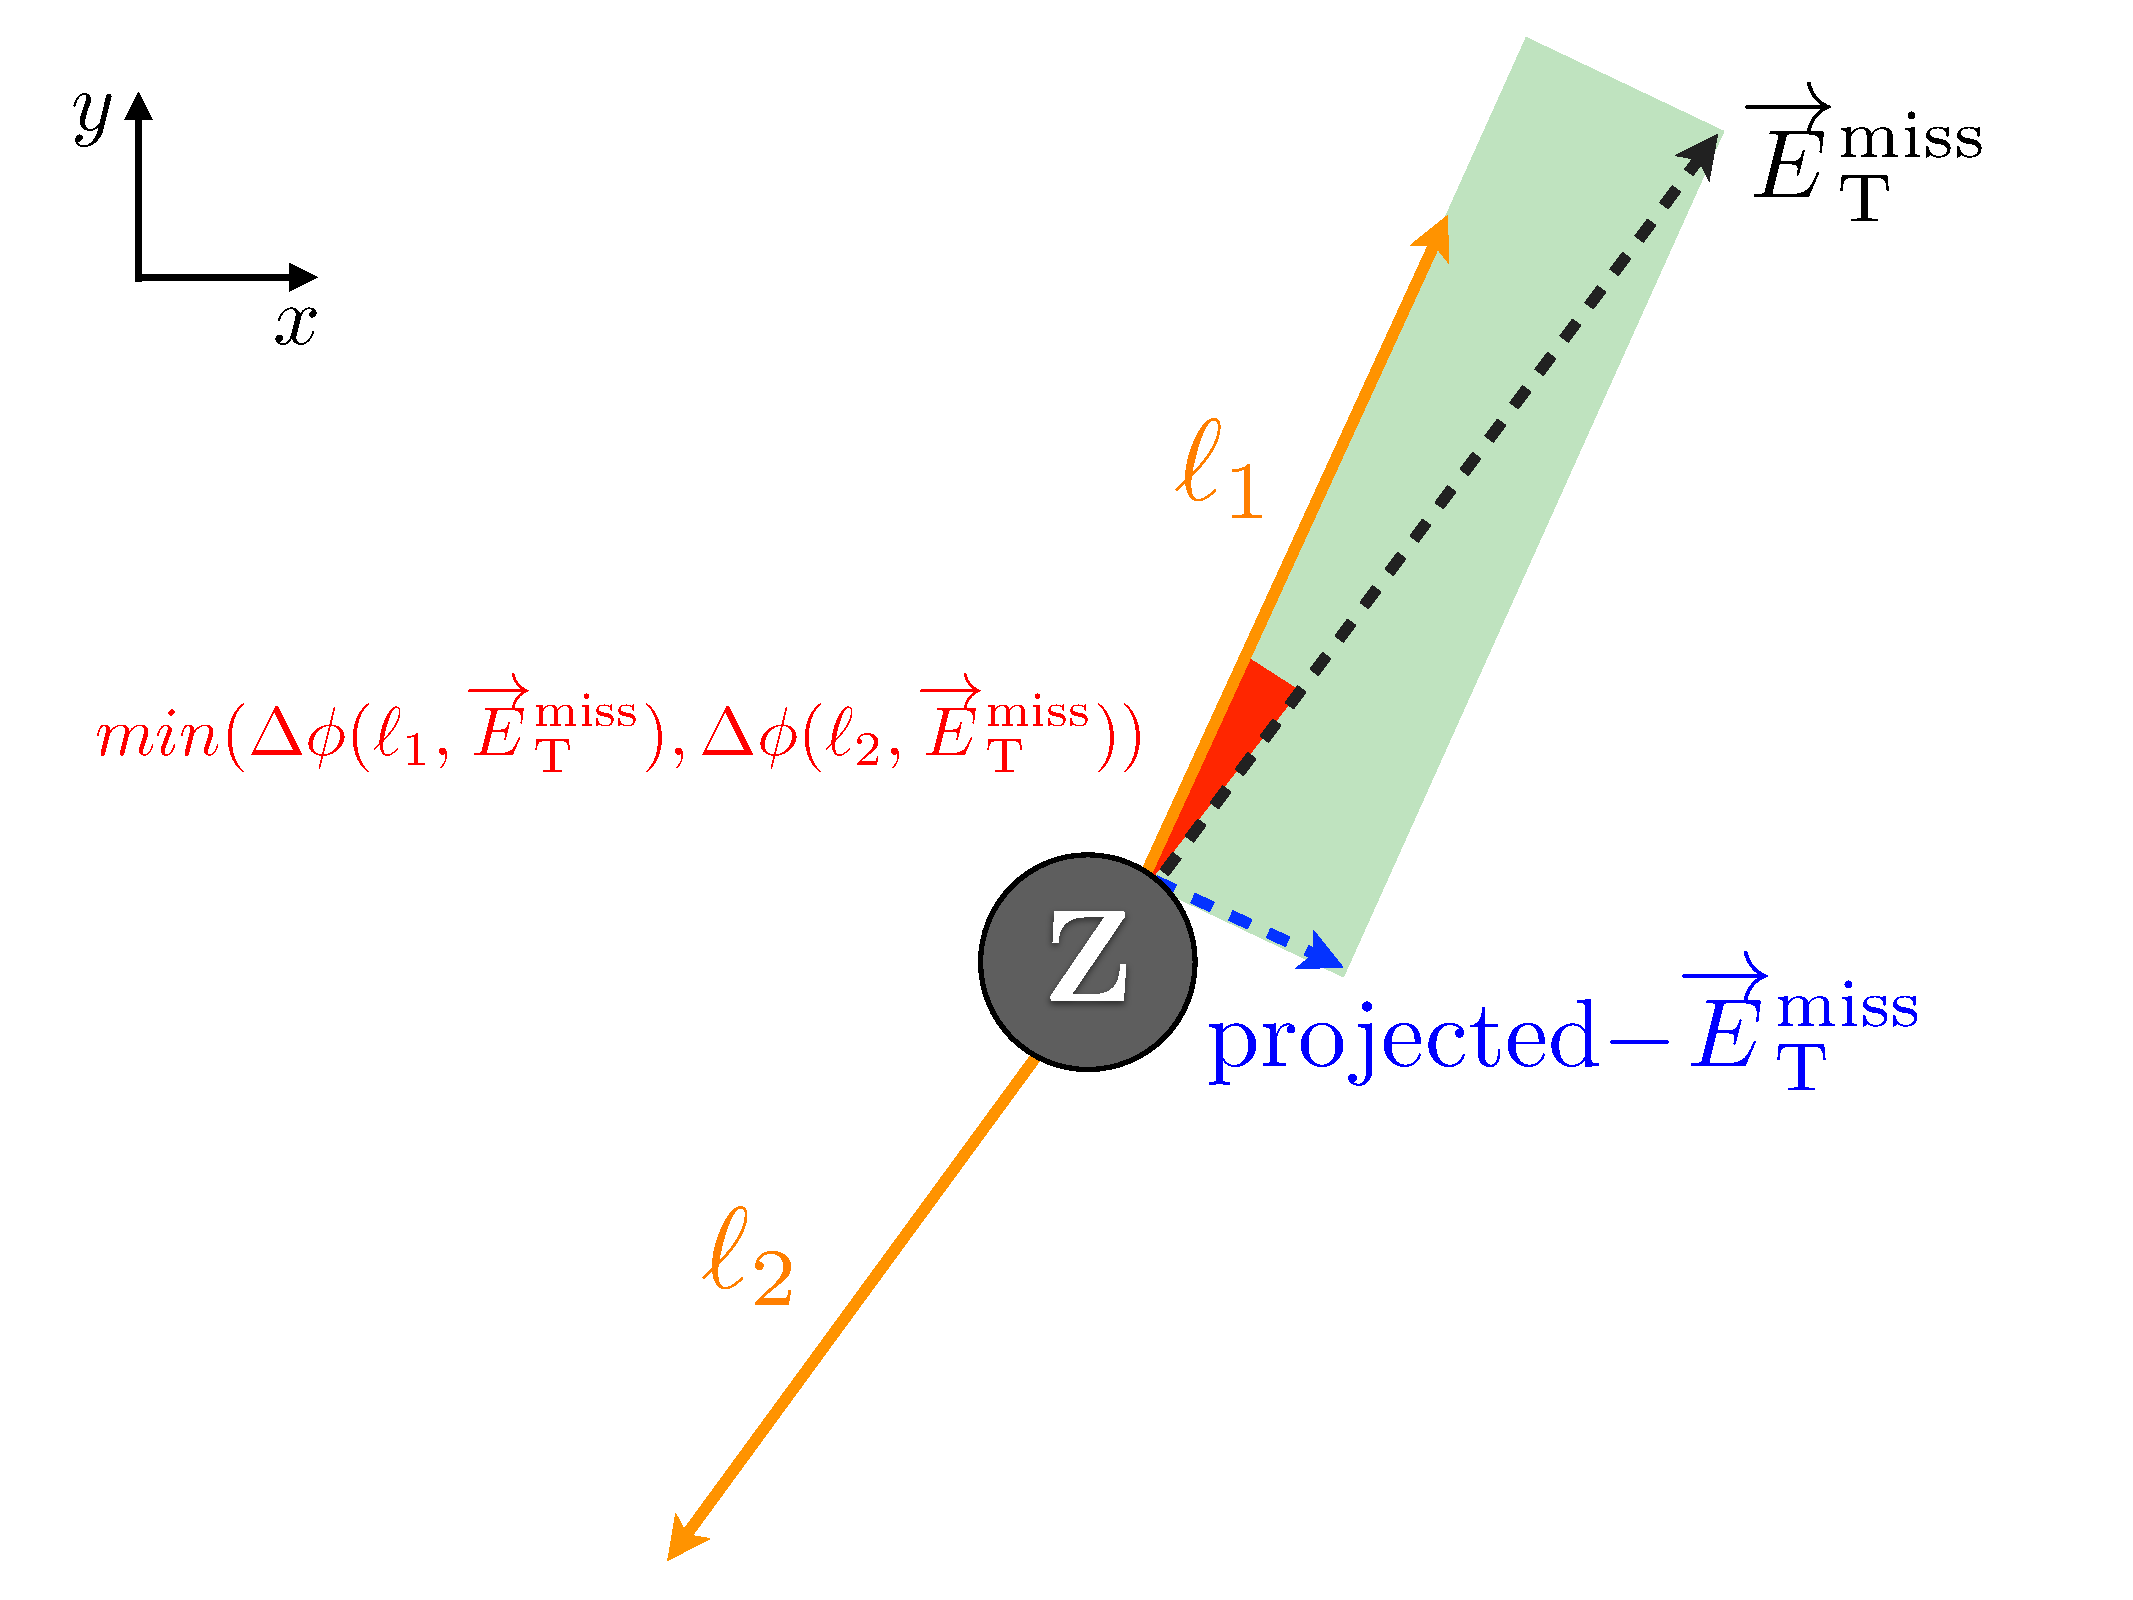
\includegraphics[width=0.7\textwidth]{figures/projmet.pdf} 
\end{tabular} 
\caption{Schematic of \pmet.}
\label{fig:projmetscheme} 
\end{figure}  
%
\begin{figure}[htp] 
\centering 
\begin{tabular}{c} 
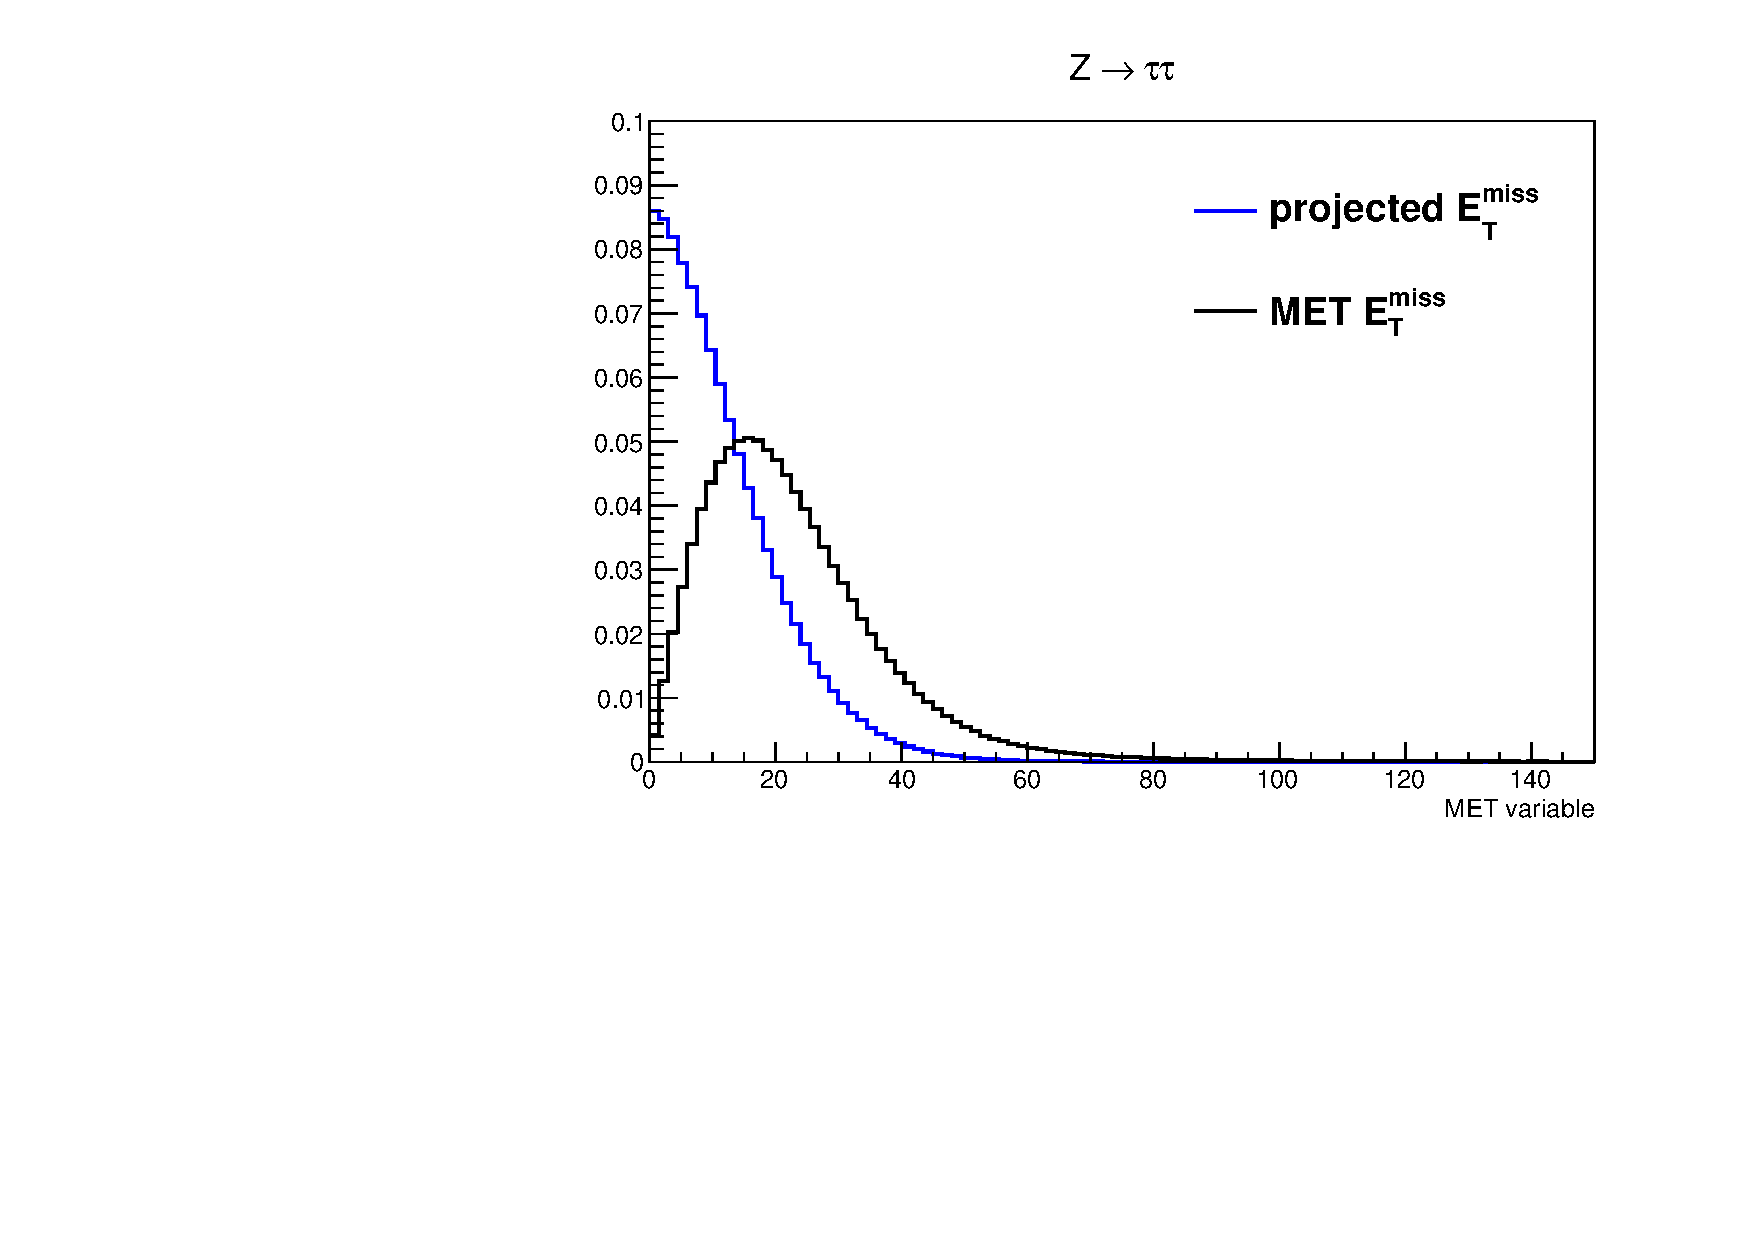
\includegraphics[width=0.45\textwidth]{figures/pmet_met_ztt.pdf} 
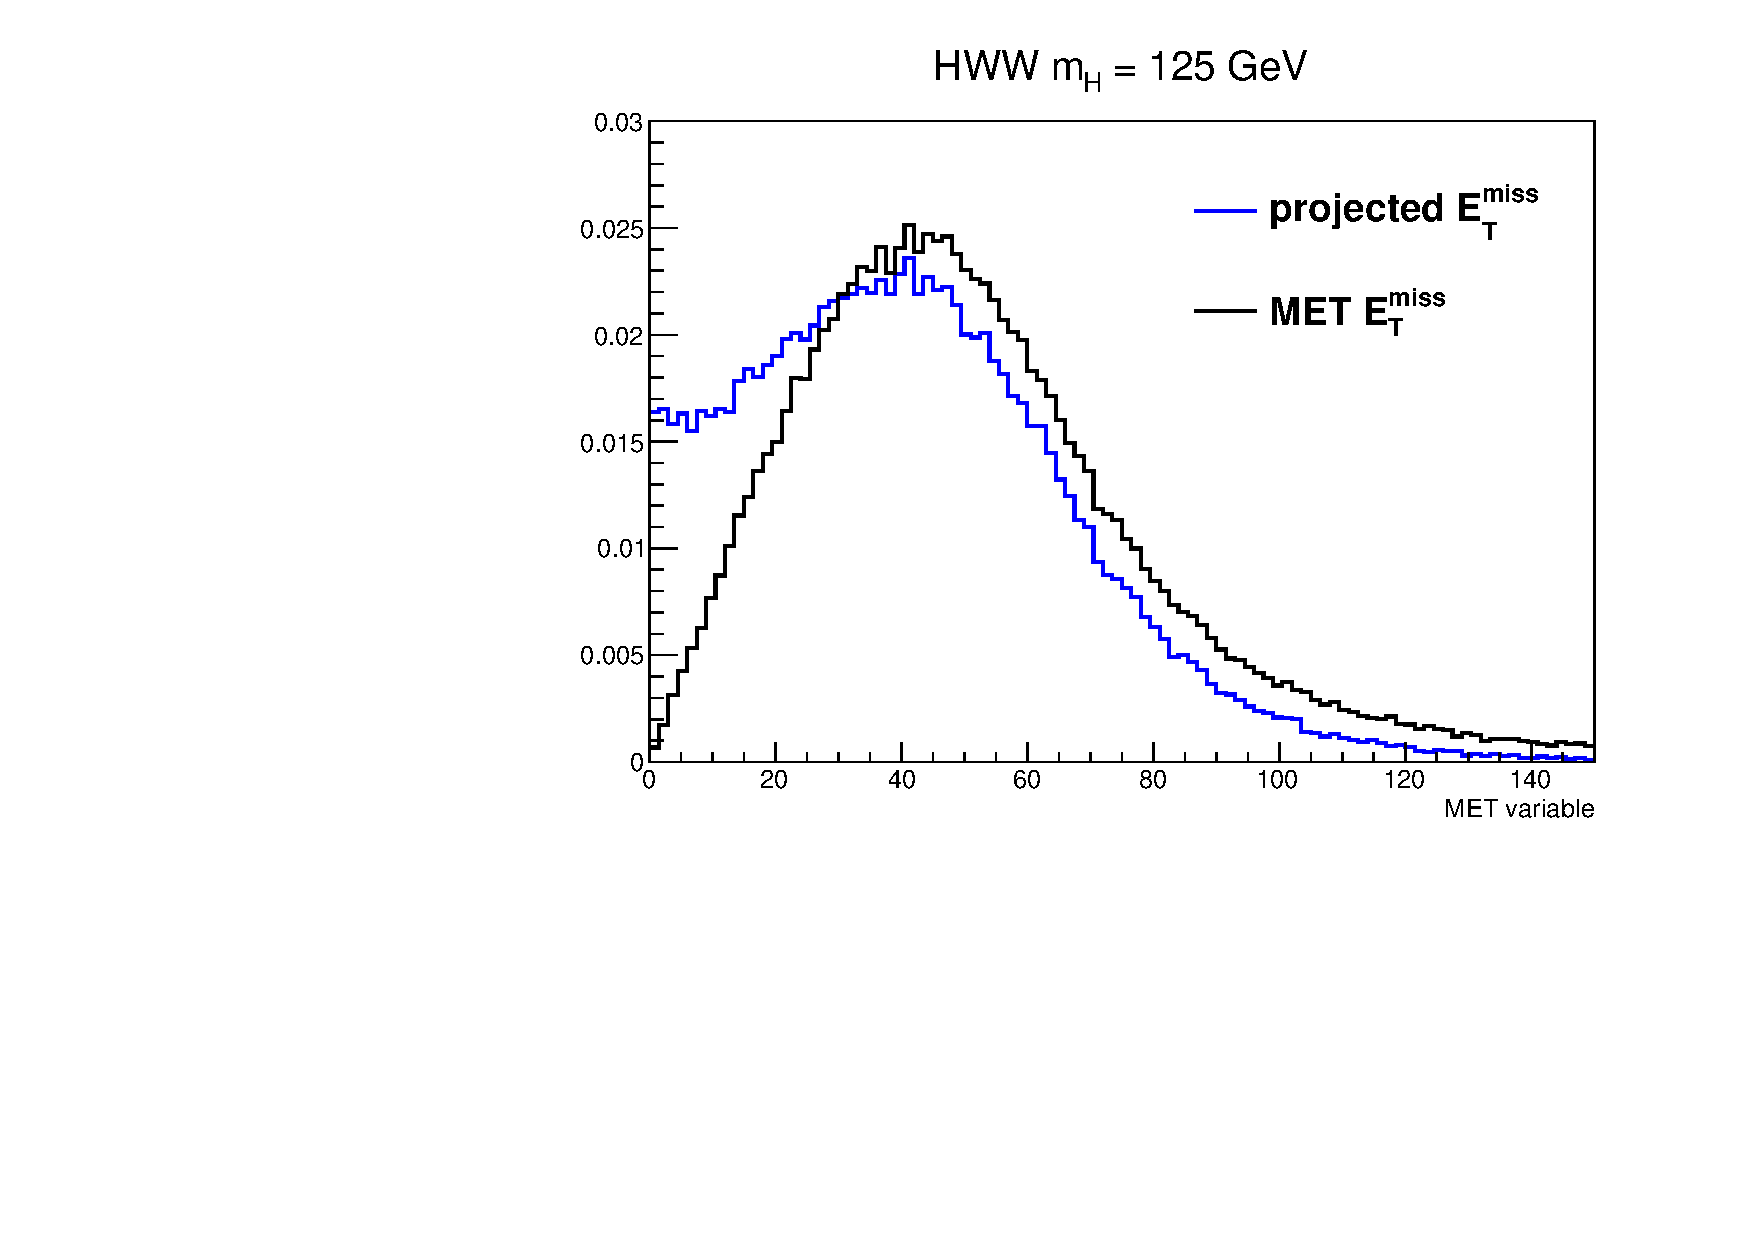
\includegraphics[width=0.45\textwidth]{figures/pmet_met_hww125.pdf} 
\end{tabular} 
\caption{\met(black) and \pmet(blue) in \dytt(left) and SM Higgs at \mHi=125~\GeV(right).}
\label{fig:projmet} 
\end{figure}  
Figure~\ref{fig:projmet} shows the \met\ and the \pmet\ distributions 
in black and red, respectively, in \dytt\ and SM Higgs at \mHi=125~\GeV\
on left and right, respectively. We can see that \pmet is more squeezed to 
the lower values in case of \dytt, giving better rejection power.  

The \trkmet\ is a variable insensitive to the pileup, 
but a drawback is that its tail is longer than \pfmet\ in the \dyll\ events. 
By isospin symmetry the average number of neutral hadrons should 
be same as that of the charged hadrons. But, if there is an imbalance between neutral 
and charged components in the jets, the \trkmet\ can be calculated arbitrarily high. 
For example, for a di-jet event with back-to-back 30~\GeV\ jets where one jet is composed 
of 10~\GeV\ of charged components and 20~\GeV\ of neutral components, and the other jet 
has the opposite composition, the \pfmet\ is 0 while \trkmet\ is 10~\GeV. 
Therefore, we use the minimum of \pfmet\ and \trkmet\, 
\begin{eqnarray} 
\minpmet = min \left( \pmet, \ptrkmet \right), 
\end{eqnarray} 
as a \met\ variable to protect \trkmet\ from those fluctuations. 
The other advantage of taking the minimum is that the the correlation 
between the two \met\ definitions is strong in the events with true \met, 
while weak in the events with fake \met\ as shown in Fig.~\ref{fig:2dmet}. 
So, by taking the minimum of them, we can get additional rejection 
of \dyll\ backgrounds without a harm to the signal.  
%
\begin{figure}[htp] 
\centering 
\begin{tabular}{c} 
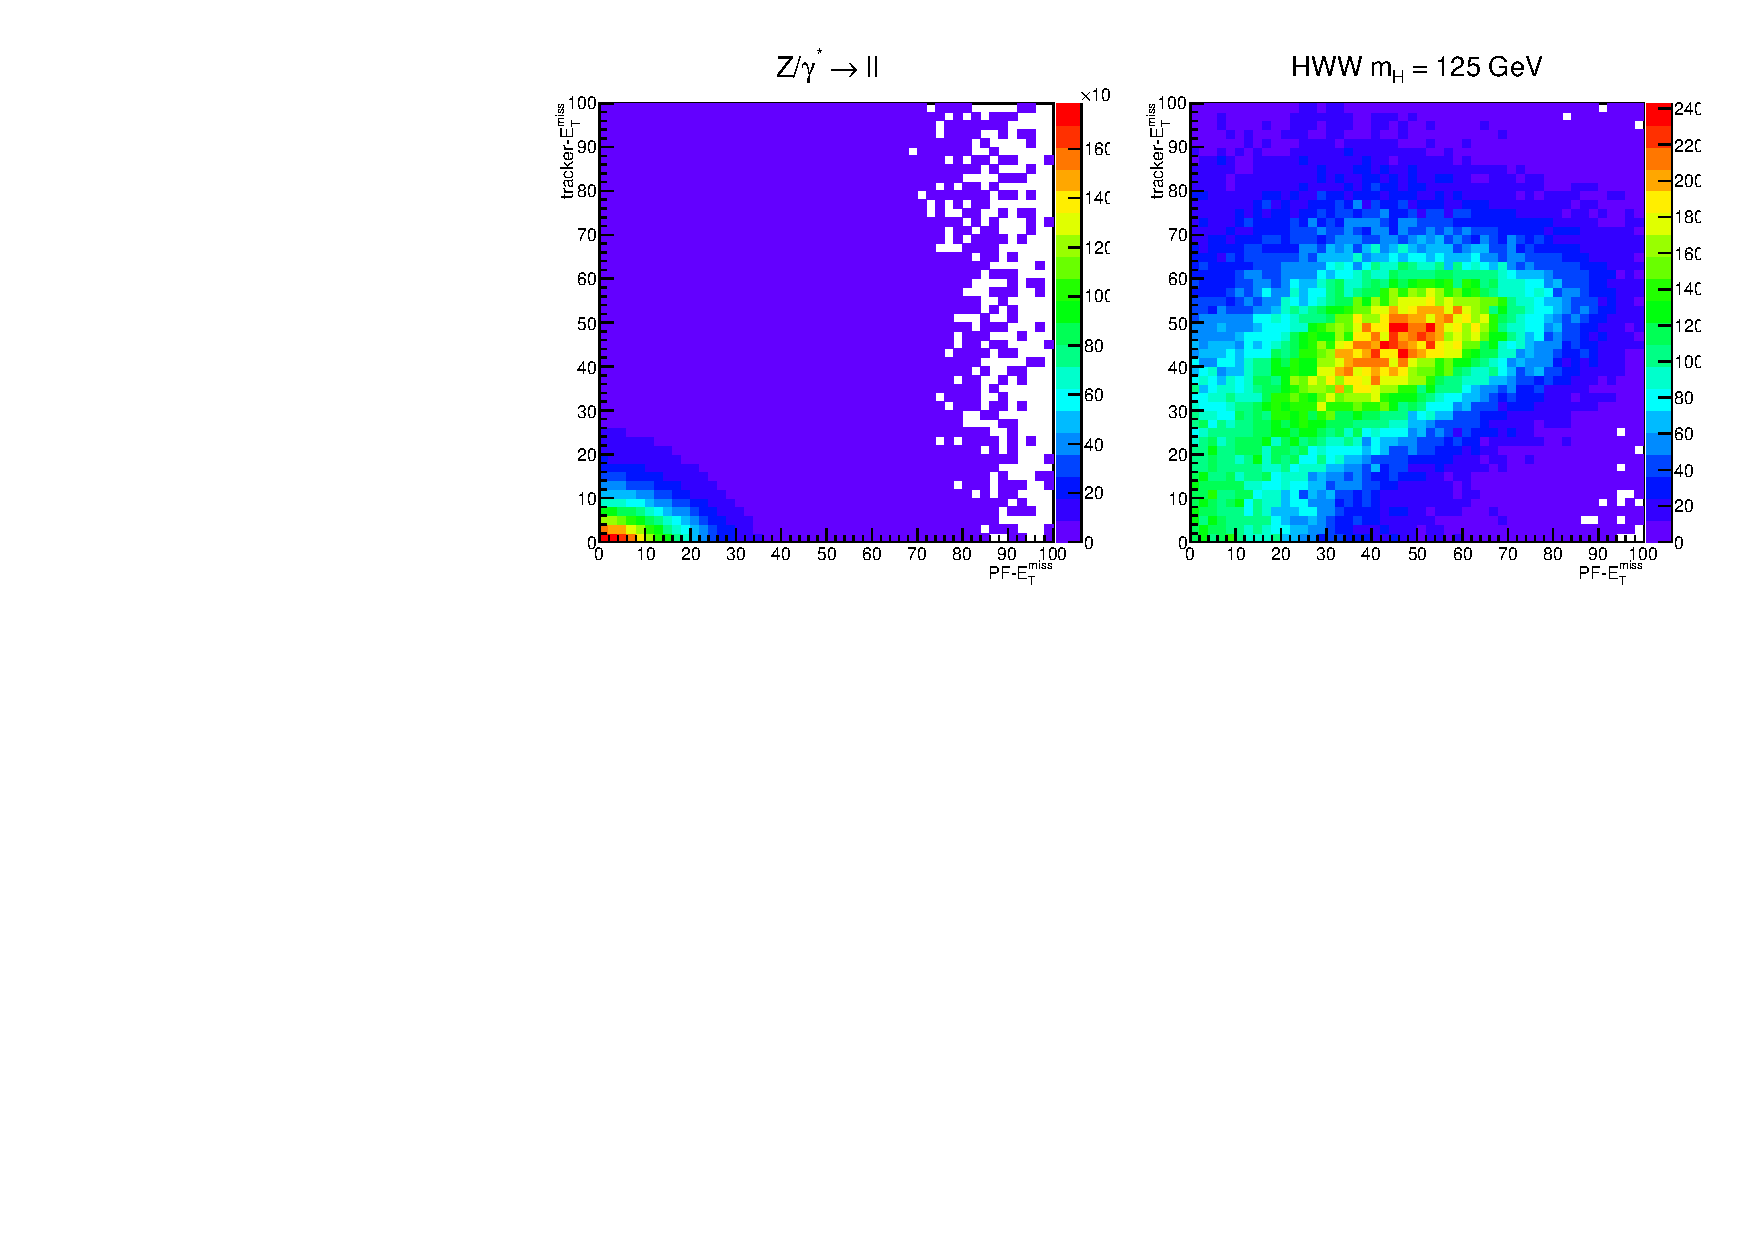
\includegraphics[width=0.99\textwidth]{figures/2dmet.pdf} 
\end{tabular} 
\caption{\pmet\ vs. \ptrkmet\ in \dyll\ and SM Higgs \mHi = 125~\GeV.}
\label{fig:2dmet} 
\end{figure}  

We require \minpmet\ to be greater than 20~\GeV\ as a baseline selecion. 
For further rejection of \dyll\ background, we apply BDT-based technique which will be 
discussed in detail in section~\ref{sec:dybkg}. 

%%%%%%%%%%%%%%%%%%%%%%%%%%%%%%%%%%%%%%%%%%%%%%%%%%%%%%%%%%%%%%%%%%
\section{ Top-tagging }

The \topbkg\ events contain additional b quarks on top of 
the two leptons and \met. The b quarks are then hadronized to B mesons, 
and develop hadronic showers. Experimentally,  
they can be identified by finding a displaced secondary vertex, B-tagging,
or a soft muon decayed from the B meson. 

The section~\ref{sec:btagging} described how the discriminator for b-tagging is constructed. 
If the b-tagging discriminator(TCHE) of a jet that passes 
the jet selection criteria described in section~\ref{sec:jetselection} 
is greater than 2.1, this jet is selected as a b-tagged jet. 
The event is rejected if there is at least one b-tagged jet. 
%\textcolor{red}{show MC vs Data of the discriminating variable in the top control region?}

We enhance the rejection of \topbkg\ backgrounds by removing events that contain 
non-isolated soft muons from heavy flavor decays. The following requirements are imposed to 
select soft muons. 
\begin{itemize} 
    \item $\pt > 3~\GeV$ 
    \item The muon should be a tracker muon,
    \item The muon should have at least two muon segments one of which is 
          in the outermost muon stations are matched,
    \item $N_{\textrm{track layers}}>5$,
    \item $|d_{0}| < 0.2$~\cm,
    \item $|d_{z}| <0.2$~\cm, and
    \item ${\rm{Iso}_{\textrm{Total}}}/{\pt}>0.1$ if $\pt>20~\GeV$
\end{itemize} 
where $N_{\textrm{track layers}}$ is the number of tracker layers where the muon track has hits, 
$d_{0}$($d_{z}$) are the transverse(longitudinal) impact parameter with respect to 
the event primary vertex, and $\rm{Iso}_{\textrm{Total}}$ is the sum of \Et\ inside of the cone 
with $dR < 0.3$ in ECAL and HCAL, and \pt\ of tracker. Adding soft muon requirement 
especially helps in the 0-jet category where the top rejection increases 
about 50 \% compared to using b-tagging only.

The total top rejection using both methods when applied to \topbkg\ MC 
is about 50 \% in the 0-jet category and 80 \% in the 1-jet category. 


\section{\dyll\ suppression in \SF\ final states} 
\label{sec:dybkg}

In the \SF\ channel, \dyll\ is one of the dominant backgrounds, 
and it is suppressed by rejecting events that have 
di-lepton mass around the Z mass. So, we veto events with 
$\left|\mll - \mZ \right| < 15~\GeV$. However, since the 
production rate of \dyll\ process is very large, even after
rejecting those events, there remains a significant contribution. 
To further reject this background, a tight \met\ requirement is typically imposed
because the \met\ in \dyll\ tends to be smaller than 
the \met\ in the signal process. 
This is because there is no genuine source of \met\ in the \dyll\ events. 
In addition to \met\ there are some difference in event kinematics.
For example, in \dyll, the di-lepton system and the leading jet tend 
to be back-to-back while in the signal events they do not have such 
correlation because there is additional degree of freedom from neutrinos.   

Usually, \dyll\ background is suppressed by applying a strong \met\ selection. 
But, this can lead to a significant loss in signal. 
So, we developed a BDT-based \dyll\ suppression technique~\cite{dymva} to recover the 
loss in the signal efficiency. 
The training is done with a combination of signal samples, \mHi = 125 and 200~\GeV, 
for signal and \dyll\ MC for background. The motivation of using a combination of the two 
\mHi\ points is to use one training for all \mHi\ points. The \DF\ events 
are used in the training because there should not be any difference in the training 
variables between \SF\ and \DF\ events. 
As a background sample, 
a combination of the Madgraph and the Powheg samples is used to maximize statistics. 
For the training, we apply the WW selection which is defined in section~\ref{sec:wwsel}) 
for the cut-based analysis
which is discussed in sec~\ref{sec:wwsel}.
The training is done separately in the 0-jet and 1-jet categories. 

The input variables to the BDT are the following. 
\begin{itemize}

%
\item \met-related variables
\begin{itemize}
\item \pmet 
\item \ptrkmet  
\item \met\ significance($\met / \sqrt{\sum_{i}^{\textrm{All objects}} E_T(i)}$
      where $E_T(i)$ is the transverse energy of the object i used for \met\ calculation) : this 
      variable is a measure of goodness of \met\ measurement, \textit{i.e.}, being small 
      means good measurement. This variable is small for signal where real \met\ is present
      and large for \dyll\ where \met\ comes from primarily mis-measurement of jet energy. 
\end{itemize}

%
\item kinematic variables
\begin{itemize}
\item Di-lepton \pt(\ptll) : this variable tends to larger for \dyll\ than signal because 
      \pt\ of the trailing lepton is softer in signal because it comes from virtual W
      with much smaller mass.

\item Higgs transverse mass($\mT=\sqrt{2\ptll\met(1-cos(\Delta\phi_{\ell\ell-\met}))}$) : 
      signal tends to have larger value because it has larger \met\ and the azimuthal 
      angle difference between di-lepton system and \met\ is smaller due to spin-0ness 
      of Higgs boson and the V-A nature of the W decay which is discussed in 
      subsection~\ref{subsec:angular_dist}.

\item leading jet \pt : this variable is larger for \dyll\ because di-lepton system 
      and the leading jet are more likely to be back-to-back and the cut on \ptll($>45~\GeV$)  
      selects events with higher jet \pt. 

\item recoil of the di-lepton + \met\ system(the magnitude of the vector sum of 
      \pfmet\ and the di-lepton system) : this variable is smaller for signal because 
      the azimuthal angle difference between di-lepton system and \met\ is smaller.

\end{itemize}

%
\item azimuthal angle differences 
\begin{itemize}
\item Azimuthal angle difference between di-lepton system and leading jet($\pt>15~\GeV$) : 
      this variable is close to $\pi$ for \dyll\ because leading jet recoils off the Z boson 
      which decays into two leptons. For signal it is less back-to-back because of additional
      degrees of freedom from neutrinos. 

\item Azimuthal angle difference between leading jet ($\pt>15~\GeV$) and \met\ :
      this variable is close to 0 for \dyll\ because \met\ mostly comes from mis-measurement 
      of jet energy. For signal it is more broad because \met\ and jet do not have 
      topological correlation due to additional degrees of freedom from leptons.


\item Azimuthal angle difference between di-lepton system and \met\ : This variable is close 
      to $\pi$ for both signal and \dyll\ because for signal the azimuthal angle difference 
      between di-lepton system and \met\ is large and for \dyll\ \met\ is aligned with jet 
      \pt\ and it is back-to-back with \ptll. But, it has different correlations for signal 
      and \dyll\ with other input variables such as azimuthal angle difference between 
      leading jet and \met.
      
\end{itemize}

%
\item other variable
\begin{itemize}
\item Number of reconstructed vertices($N_{vtx}$) : This variable has different correlations for 
      signal and \dyll\ with other input variables. For example, for \dyll\ \met\ has a 
      large correlation with $N_{vtx}$ because the more interaction are present, the worse 
      jet energy resolution becomes, thus \met\ becomes large. But, for signal, \met\ is 
      less affected by pileup because the magnitude of additional contribution from 
      pileup events is very small compared to the real \met\ caused by neutrinos. 

\end{itemize}

\end{itemize}

\begin{figure}[htp] 
\centering
\begin{tabular}{c} 
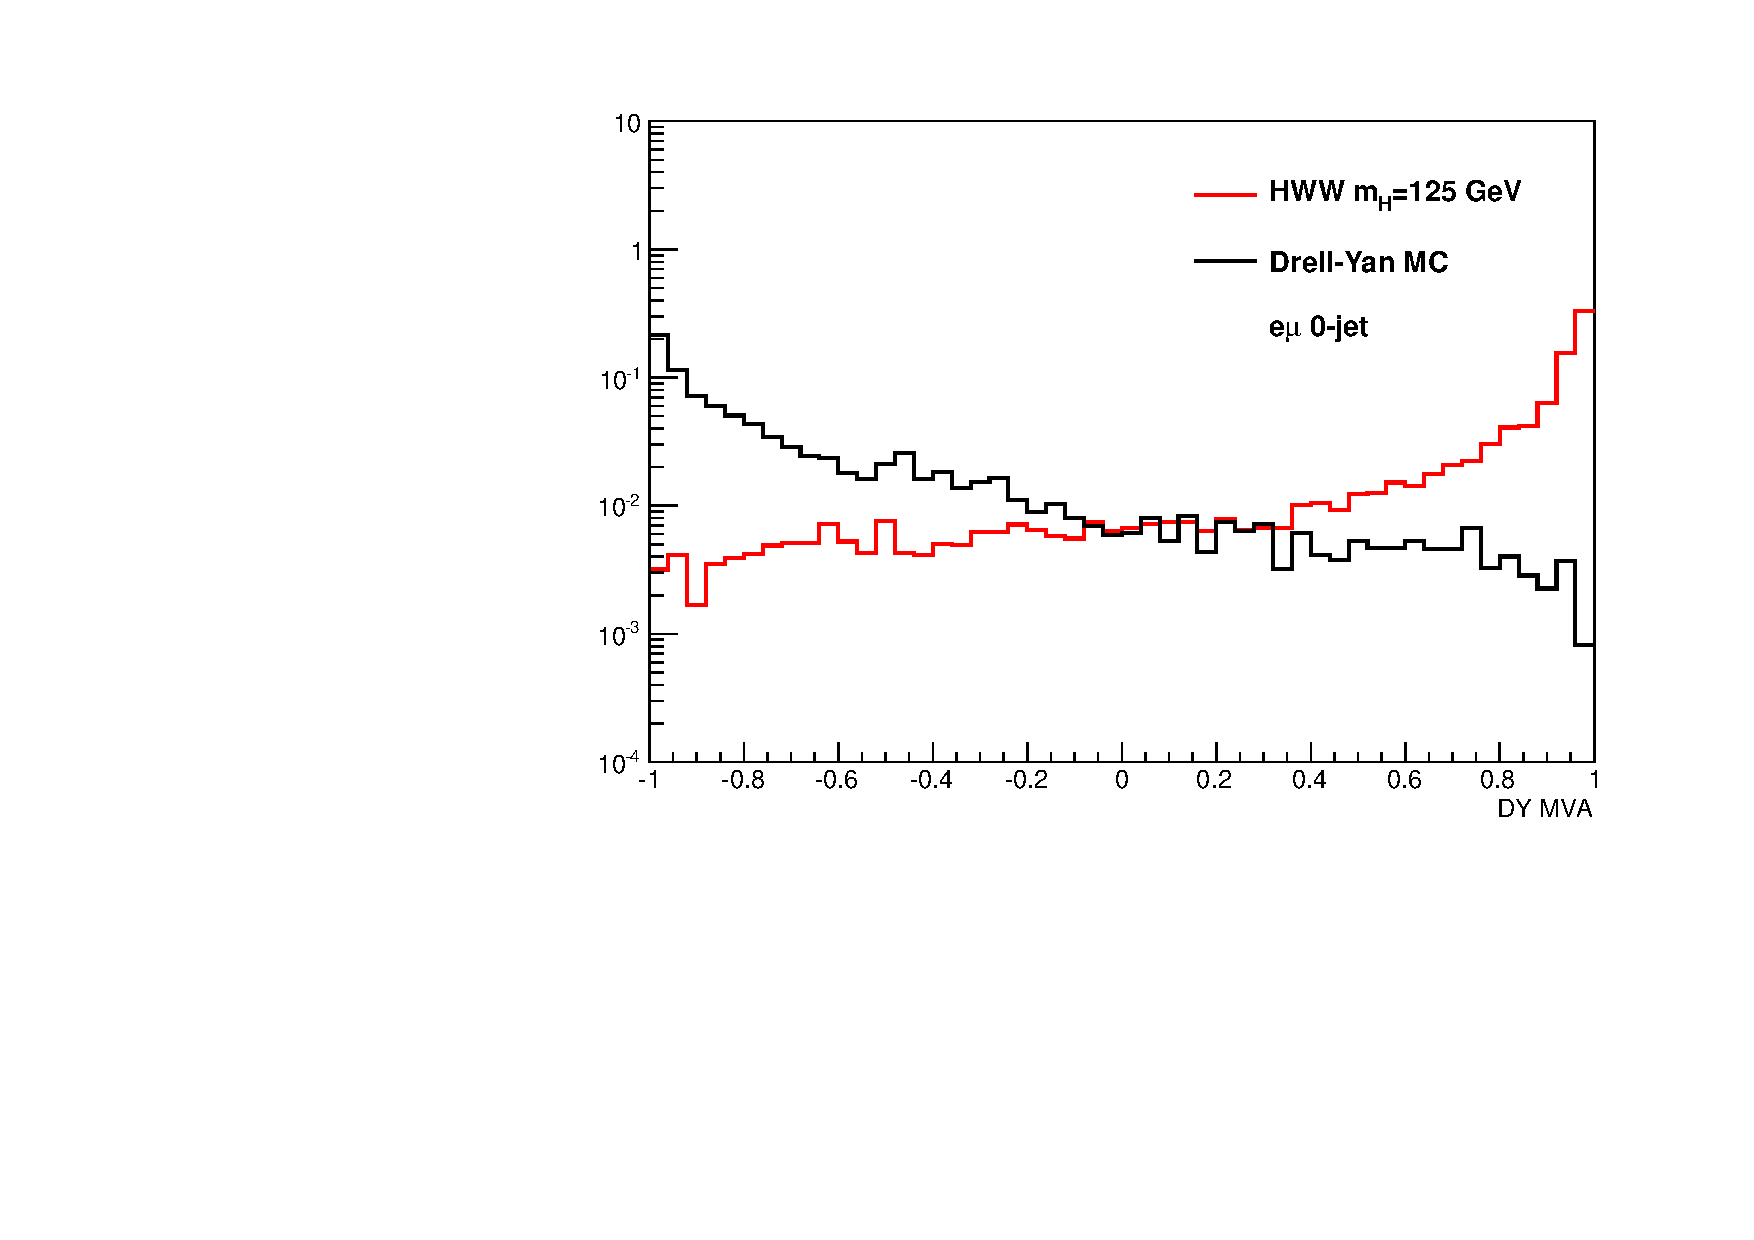
\includegraphics[width=0.5\textwidth]{figures/dymva_0j.pdf} 
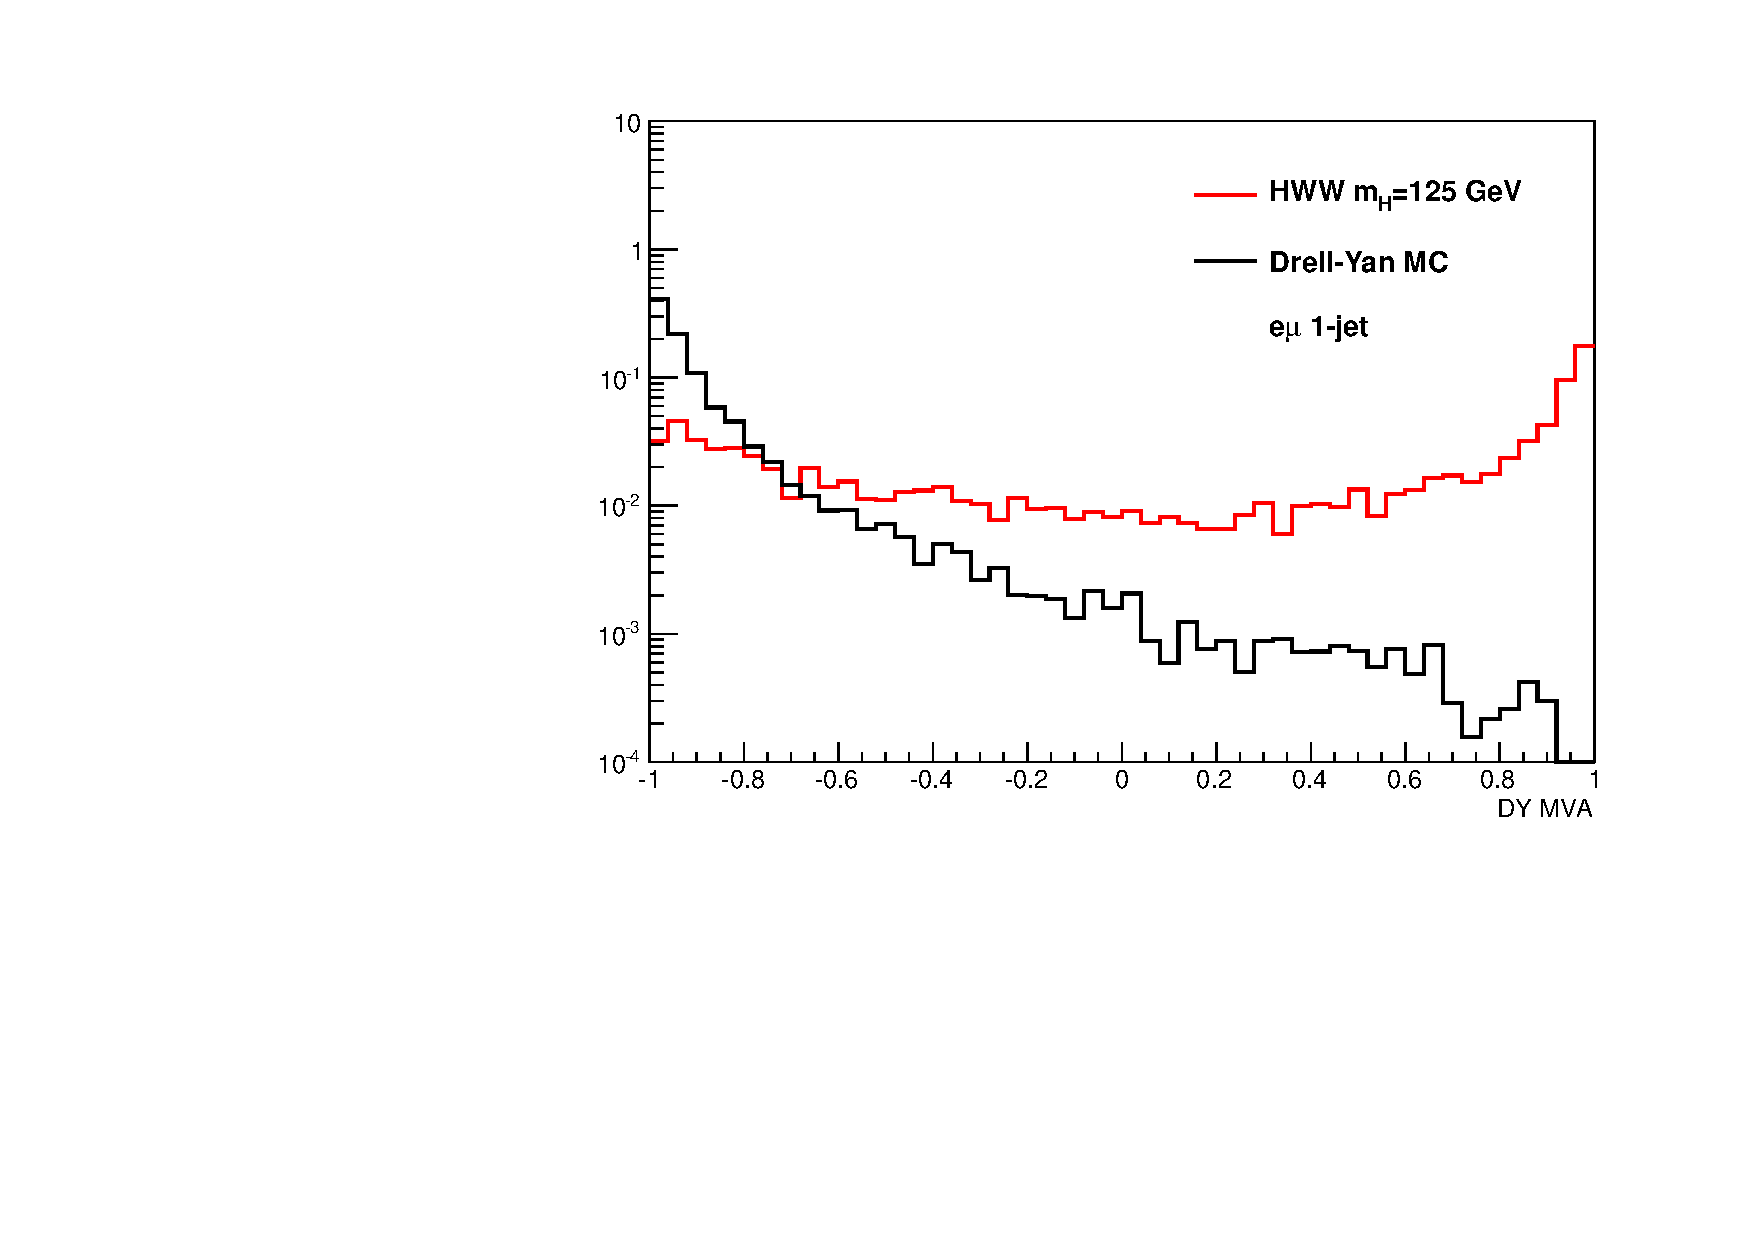
\includegraphics[width=0.5\textwidth]{figures/dymva_1j.pdf} 
\end{tabular} 
\caption{The BDT score for \mHi = 125~\GeV(red) and \dyll\ MC(black)
in 0-jet(left) and 1-jet(right) categories.} 
\label{fig:dymva} 
\end{figure} 

Figure~\ref{fig:dymva} shows the BDT scores for \mHi = 125~\GeV in red 
and \dyll\ MC in black in 0-jet(left) and 1-jet(right) categories. We finally require 
that the BDT score be greater than 0.88(0.84) in 0-jet(1-jet) category. 
This requirement is applied to only \SF\ category. 
The signal(\mHi=125~\GeV) efficiency of this selection is 50~\% and 35~\% 
in 0-jet and 1-jet categories, respectively, 
and the background(\dyll\ MC) efficiency is 0.5~\% and 0.1~\% in 0-jet and 1-jet categories
%The \DF\ category has only $\minpmet>20~\GeV$ requirement.

\section{Additional Selections}

To reject events with more than two leptons such as \vv\ where both bosons decay leptonically, 
we veto events if they contain a third lepton with $\pt>10~\GeV$. 
This requirement rejects about 30~\% of events containing more then two leptons in \vv. 

At low \mll\ region, there are multiple resonances such as 
$\Upsilon$($m_\Upsilon\sim 10~\GeV$) and $J/\psi$($m_{J/\psi}\sim 3~\GeV$).
In order to reject these resonances, we apply $\mll>12~\GeV$ . 

\Wjets\ background tends to have small \ptll\ because the lepton from W and 
the recoiling jet are likely to be back-to-back. So, in order to suppress 
\Wjets\ further, $\ptll>30(45)~\GeV$ is applied for shape-based (cut-based) approaches. 

\section{WW Selection}
\label{sec:wwsel}
All requirements imposed so far are designed to select events containing 
a pair of W. This baseline selection is called ``WW selection" and 
the stage of selection where the WW selection is applied is called ``WW level".
By applying WW selection, we can reach better signal-to-background ratio(S/B),
therefore a reasonable extraction of signal becomes possible. 
Table~\ref{tab:wwselection} summarizes the requirements of the WW selection. 

\begin{table}[htp] 
\begin{center} 
\begin{tabular}{c|cc}
\hline
Selection & \DF & \SF \\
\hline \hline 
\ptlmax & $>20~\GeV$ & $>20~\GeV$ \\
\ptlmin & $>10~\GeV$ & $>10~\GeV$ \\
Lepton selection & applied & applied \\
Number of jet selection & applied & applied \\
Third lepton veto & applied & applied \\
opposite-sign requirement & applied & applied \\
\mll & $>12~\GeV$ & $>12~\GeV$ \\
$\left| \mll - m_Z \right| > 15~\GeV$ & not applied & applied \\
\minpmet & $>20~\GeV$ & $>20~\GeV$ \\
BDT-based Drell-Yan suppression & not applied & applied \\
Top veto & applied & applied \\
\ptll & $>30~\GeV$[*] & $>45~\GeV$ \\
\hline
\end{tabular} 
\caption{Summary of WW selection. [*] For shape-based method 
$\ptll>30~\GeV$ is applied and for cut-based method $\ptll>45~\GeV$ is applied.}
\label{tab:wwselection} 
\end{center} 
\end{table} 


